%%% Kapitoly
\chapter{Experimenty}
\section{Úvod}
Všechny práce zmíněné v úvodní kapitole, sice používají evolučních algoritmů k vytvoření řízení chování homogenního robotického hejna, tzn. s pouze jedním druhem robotů. Cílem této práce je najít použití evolučních algoritmů i pro heterogenní hejna. Následující části mají přiblížit obecný postup při hledání optimálního chování hejn, stručně popsat jednotlivé experimenty a poté podrobněji rozebereme každý  experiment zvlášť.
\par 
\subsection{Experimenty}
Pro testování jsem zvolil tři rozličné scénáře. Hlavní motivací bylo jednotlivé úkoly pro hejno udělat komplexnější, aby každá skupina robotů byla schopna řešit pouze část ze zadání scénáře. Také jsem se snažil, aby se scénáře blížily reálným situacím z reálného světa.\par 
\textbf{Pracovní názvy}
\begin{enumerate}
	\item Wood Scene
	\item Mineral Scene
	\item Competitive Scece
\end{enumerate}
\subsubsection{Wood Scene}

\subsubsection{Mineral Scene}
Jedná se o scénář reprezentující sběr surovin pro výrobu paliva a jeho následné využití. Figurují zde 3 rozliční roboti, všichni potřebují pro pohyb  dané množství paliva. Úspěšnost daného hejna se měří množstvím paliva. Nejmenší robot(Mineral scout) disponuje pouze senzory k exploraci prostředí a rádiovým vysílačem pro komunikaci se skupinou. Robot prostřední velikosti(Mineral Worker) se pohybuje o něco pomaleji než Mineral Scout, ale umí přesouvat objekty i více najednou. Robot pro přeměnu minerálu(,suroviny na výrobu paliva,) označen ve frameworku jako Mineral Refactor se přemisťuje nejpomaleji, má možnost přeměnit minerál na palivo. Tento scénář si bere jako inspiraci strategické hry a hypotetické přežití robotů na cizí planetě, kde si budou muset obstarat vlastní 
nerostné suroviny pro běh.

\subsubsection{Competitive Scene}
Poslední ze scénářů se týká soutěže dvou týmů(hejn) ve kterých figurují jeden malý průzkumný robot(Competitive Scout) a jeden vetší bojový robot(Competitive Fighter). Úspěšnost týmu je dána zachovanými jednotkami zdraví robotů a uděleným poškozením do nepřátelské skupiny robotů. Competitive Scout se pohybuje značně rychleji než Competitive Fighter, ale uděluje menší poškození. Což lze opět vztáhnout na chování rozdílných skupin nepřátel např. ve strategických hrách, kde se jejich chování adaptuje, co nejlépe na dané prostředí. 
\subsection{První Kroky}
\unsure{Pravděpodobně špatný název kapitoly}
\par
Nejvíce se budu věnovat prvnímu scénáři, protože jsem na něm strávil většinu času a testoval na něm různé postupy. Také jsem jej používal  jako benchmark pro počítání průsečíků, paralelního zpracování jednotlivých generací, v neposlední řadě sloužil pro odhalení většiny chyb simulace, návrhu vizualizace a formátu souboru pro nastavení ES,DE. Nakonec se ukázalo, že postup aplikovaný na jeho řešení je rentabilní i pro další dva scénáře. Takže pro další dva scénáře už bylo klíčové nalézt pouze fitness funkci a nastavení parametrů DS a ES.
\par
V úvodu bych se také rád zmínil o prvotních pokusech řešení problému evoluce heterogenní skupiny robotů právě na prvním ze scénářů. Nejdříve jsem pro otestování prostředí a ověření dostatečné obtížnosti testovacích scénářů zkoušel generovat náhodné neuronové sítě a po-té měřit jejich úspěšnost. Pokud jsem se soustředil pouze na hlavní úkol a roboti nebyly hodnoceny za žádné další interakce, tak žádný ani z 20 000 jedinců nedosáhl na jiné hodnocení než 0. Což prokázalo komplexnost scénářů a jich obtížnost.
\par 
Dále nastal čas vyzkoušet evoluční algoritmy pro vytvoření chování(, tzn. optimalizaci neuronové sítě). Zvolil jsem, stejně jako v předchozím případě, fitness funkci hodnotící pouze hlavní cíl scénáře. Tento postup se také ukázal opět jako nedostatečný, jelikož žádná z náhodně vytvořených neuronových sítí nebyla schopna řešit žádným způsobem (, ani velmi hloupě). Diferenciální evoluce se v tomto případě chovala velmi podobně jako "random search" algoritmus, jelikož hodnota fitness byla pro  všechny řešení 0,. Evoluční strategie měly problém se pohnout jakýmkoli směrem, protože směr prohledávání řešení je závislý na velikostech fitness. Což lze jednoduše vypozorovat z definice algoritmu v kapitole \ref{sec:ES} o ES. Takže i tento postup se ukázal bez jakéhokoli výsledku. \unsure{Nenapadá mě, jak kreslit graf s nulovou fitness, nakreslit vzdálenosti mezi jednotlivými neuronkami?}
\redo{Přidat tabulku s parametry funkce těchto běhů} 
\par 
Dalším vylepšením bylo přidat některé meta-úkoly, které budou jednoduché a dosažitelné i pro vygenerované algoritmy. Předpokládal jsem, že jejich postupné vylepšování evolučními algoritmy povede k řešení složitějších úkolů a nakonec až k hlavnímu cíli. Například zahrnout fitness počet navštívený částí mapy, už před připraveným objektů a podobně. V ideální případě by se měla populace blížit k ideálnímu řešení jednoho z jednodušších meta-úloh. Díky tomu by mělo být jednoduší narazit na chování řešící i složitější úlohy, protože spolu evidentně souvisí. Což můžeme ilustrovat na WoodScene scénáři, kde roboti prozkoumávající rychle a ve velké rozptylu mají možnost pokácet vícero stromů. I přes mé optimistické výhledy se ukázalo, že jedinci jsou díky složitější fitness funkci mnohem náchylnější k zaseknutí v lokálním optimu. Zasekávaly se u jednodušších úkolů, vylepšovali jen je. Nové komplexnější chování se objevilo velmi zřídka a jedinci obdařeny těmito vlastnosti opět vylepšovali pouze jednoduché chování. Pokusil jsem se zabránit zaseknutím v lokálních maximech přes různé ohodnocení fitness, ale výsledky opět neukázali přívětivé.\par
Z předchozích zkušeností jsem usoudil, že bude potřeba vytvořit nějakou postupnou cestu k řešení tolik náročného cíle. \unsure{Můžu přiznat, že mi vedoucí radí?} Na základě konzultací se svým vedoucím jsem vytvořil koncept meta-úkolů, jedná se o jednodušší úlohy vedoucí k té hlavní. Od předchozího postupu se odlišuje oddělením jednotlivých fitness funkcí odpovídající meta-úkolu. Použiji evoluční algoritmy s fitness funkcí pouze aktuálního meta-úkolu a po dosažení dostatečné úrovně splnění meta-úkolu, vezmu vytvořenou generaci a použiji na ní evoluční algoritmus s fitness soustředěnou na následující meta-úkol. Tento postup opakuji až jako fitness funkci použiji vlastní ohodnocení scénáře. Uvedený přístup konečně vedl k uspokojivým výsledkům a jednotlivé průběhy budou popsány v dalších kapitolách. \par 
Zkoušel jsem také testovat, roboty s paměťovými sloty oproti těm bez. Úspěšnost a konvergence robotů s pamětí se znatelně se učil pomaleji. Největší problém byl s tím, že robot se dostal do kolize s prostředí a pak vycouval, ale protože si nedrží žádný stav, tak znovu najel do kolize a stále dokola. Roboty bez slotů se nebyly schopni přiblížit k výsledkům těm s pamětí ani při velkém počtu generací. Z tohoto důvodu všichni roboti mají připojeno alespoň 5 paměťových slotů. Paměťový slot zároveň chová jako senzor i jako efektor. 

\section{Použité technologie}
\subsection{Reprezentace Chování}
Pro ovládání robotů jsem zvolil v poslední době velmi oblíbené neuronové sítě. Použil jsem jejich oblíbenou definici podle pánů Warren S. McCulloch a  Walter Pitts \citep{neuron}, kteří ji prezentovali už v roce 1943. 
\begin{itemize}[]
	\item $n$: velikost vstupu
	\item $x_i$:  i-tý vstup neuronu
	\item $w_i$:  váha i-tého vstupu
	\item $\Theta$: práh, (váha s konstatním vstupem 1)
	\item $S(x)$: přenosová funkce
	\item $Y$: výstup neuronu 
\end{itemize}

\begin{center}
	\large{\boldsymbol{$Y = S(\Theta + \sum_{i=0}^{n} w_i x_i)$}}
\end{center}
\improvement{Přidat obrázek funkce.}Jako aktivační funkce se mi nejvíce osvědčila často používaná funkce hyperbolického tangentu se změněným oborem hodnot pro konkrétní výstup. \par
\unsure{To úplně nevím, zda je pravda}Jelikož v mé práci bylo prioritou nalézt funkční řešení jednotlivých scénářů a nikoliv optimalizaci pro co nejlepší výsledek.  Zvolil jsem jednoduchou architekturu jednovrstvé neuronové sítě, což se ukázala jako dostatečné. Takže pro každé reálné číslo, které očekává robot jako vstup pro efektor, byl připojen neuron do kterého vstupuje vektor reálných čísel odpovídající každé hodnotě ze senzorů.  Pro ještě lepší řešení by zde bylo možné nasadit NEAT algoritmus či hledat více specifičtější architektur, případně vyzkoušet vliv vícero vrstev. \unsure{Mohu to napsat sem? nebo do diskuze}
\subsection{Evoluční algoritmy}
Neuronovou sítě si lze představit jako množinu vektorů, kde jeden perceptron odpovídá vektoru reálných čísel(, vah vstupů + práh \boldsymbol{$v =(x_0,x_1...x_n,\Theta)$}. V kontextu evolučních algoritmů se pro optimalizaci vektorů reálných čísel nejčastěji používají Evoluční strategie a Diferenciální evoluce. I z tohoto důvodu jsem zvolil zmíněné algoritmy jako zástupce pro optimalizaci chování heterogenní skupiny robotů. Oba zmíněné algoritmy popisuji v kapitole \ref{sec:DE} a \ref{sec:ES} a má implementace se od popisu v úvodu liší pouze v malý detailech. Do detailu jsou popsány v přiložené dokumentaci. \redo{Přidat do docu}
\par
\section{WoodScene experiment}
\subsection{Cíl Experimentu}
Tento scénář je analogií pro kácení lesa, kdy se roboti snaží maximalizovat množství zpracované dřevo na předem vyznačené ploše. Plocha pro skládání dřeva je označena rádiovým signálem s hodnotou signálu 2. V experimentu se dohromady celkem vyskytuje 9 robotů dvou různých druhů. Roboti jsou na začátku simulace umístěni uprostřed mapy na skládacím prostoru. Na náhodných pozicích jsou rozmístěny stromy. Scout roboti musí nejdříve strom nalézt a zpracovat, disponují totiž efektorem zpracovávající dřevo. Ovšem Scout roboti neuvezou žádné entity, proto Worker roboti mají za úkol zpracovaný strom naložit a odvézt do skládacího prostoru.
\par
V rámci bakalářské práce byla připraven program zajišťující jednoduchou vizualizaci chování robotů. Jeho vizuální výstup můžete vidět na obrázku \ref{obr04:WoodSceneRandomStart}. Na ní si vysvětlíme jednotlivé entity nacházející se na mapě. Mapa je ohraničena čtvercovými hranicemi, které se chovají jako zeď. Zelené kroužky znázorňují stromy, které ještě nebyly objeveny. Objevený strom změní barvu na žlutou. Modře označený prostor je určen pro uskladnění zpracovaného dřeva. Hnědé kolečka zastupují pokácené dřevo. V některých pod-úkolech se objevuje dřevo už při inicializaci, proto ještě neobjevené má tmavší barvu a objevené světlejší. Pro roboty je v tomto prostoru vysílán rádiový signál. Roboti jsou vyplněny červenou barvou, jejich sensory a efektory mají černou barvu. Pro každý rádiový signál je určena jedna unikátní barva s alfa kanálem. \par
Pro potvrzení, že scénář není triviálně řešitelný. Bylo vygenerováno tisíc náhodných chování. Hodnoceny byly dle fitness funkce podúkolu kooperace popsaný níže. Nejlepší z nich můžete vidět těsně po inicializaci mapy \ref{obr04:WoodSceneRandomStart}. Výsledek krátce před 10 000 iterací je zachycen v obrázku \ref{obr04:WoodSceneRandomEnd}

\begin{figure}[p]\centering
	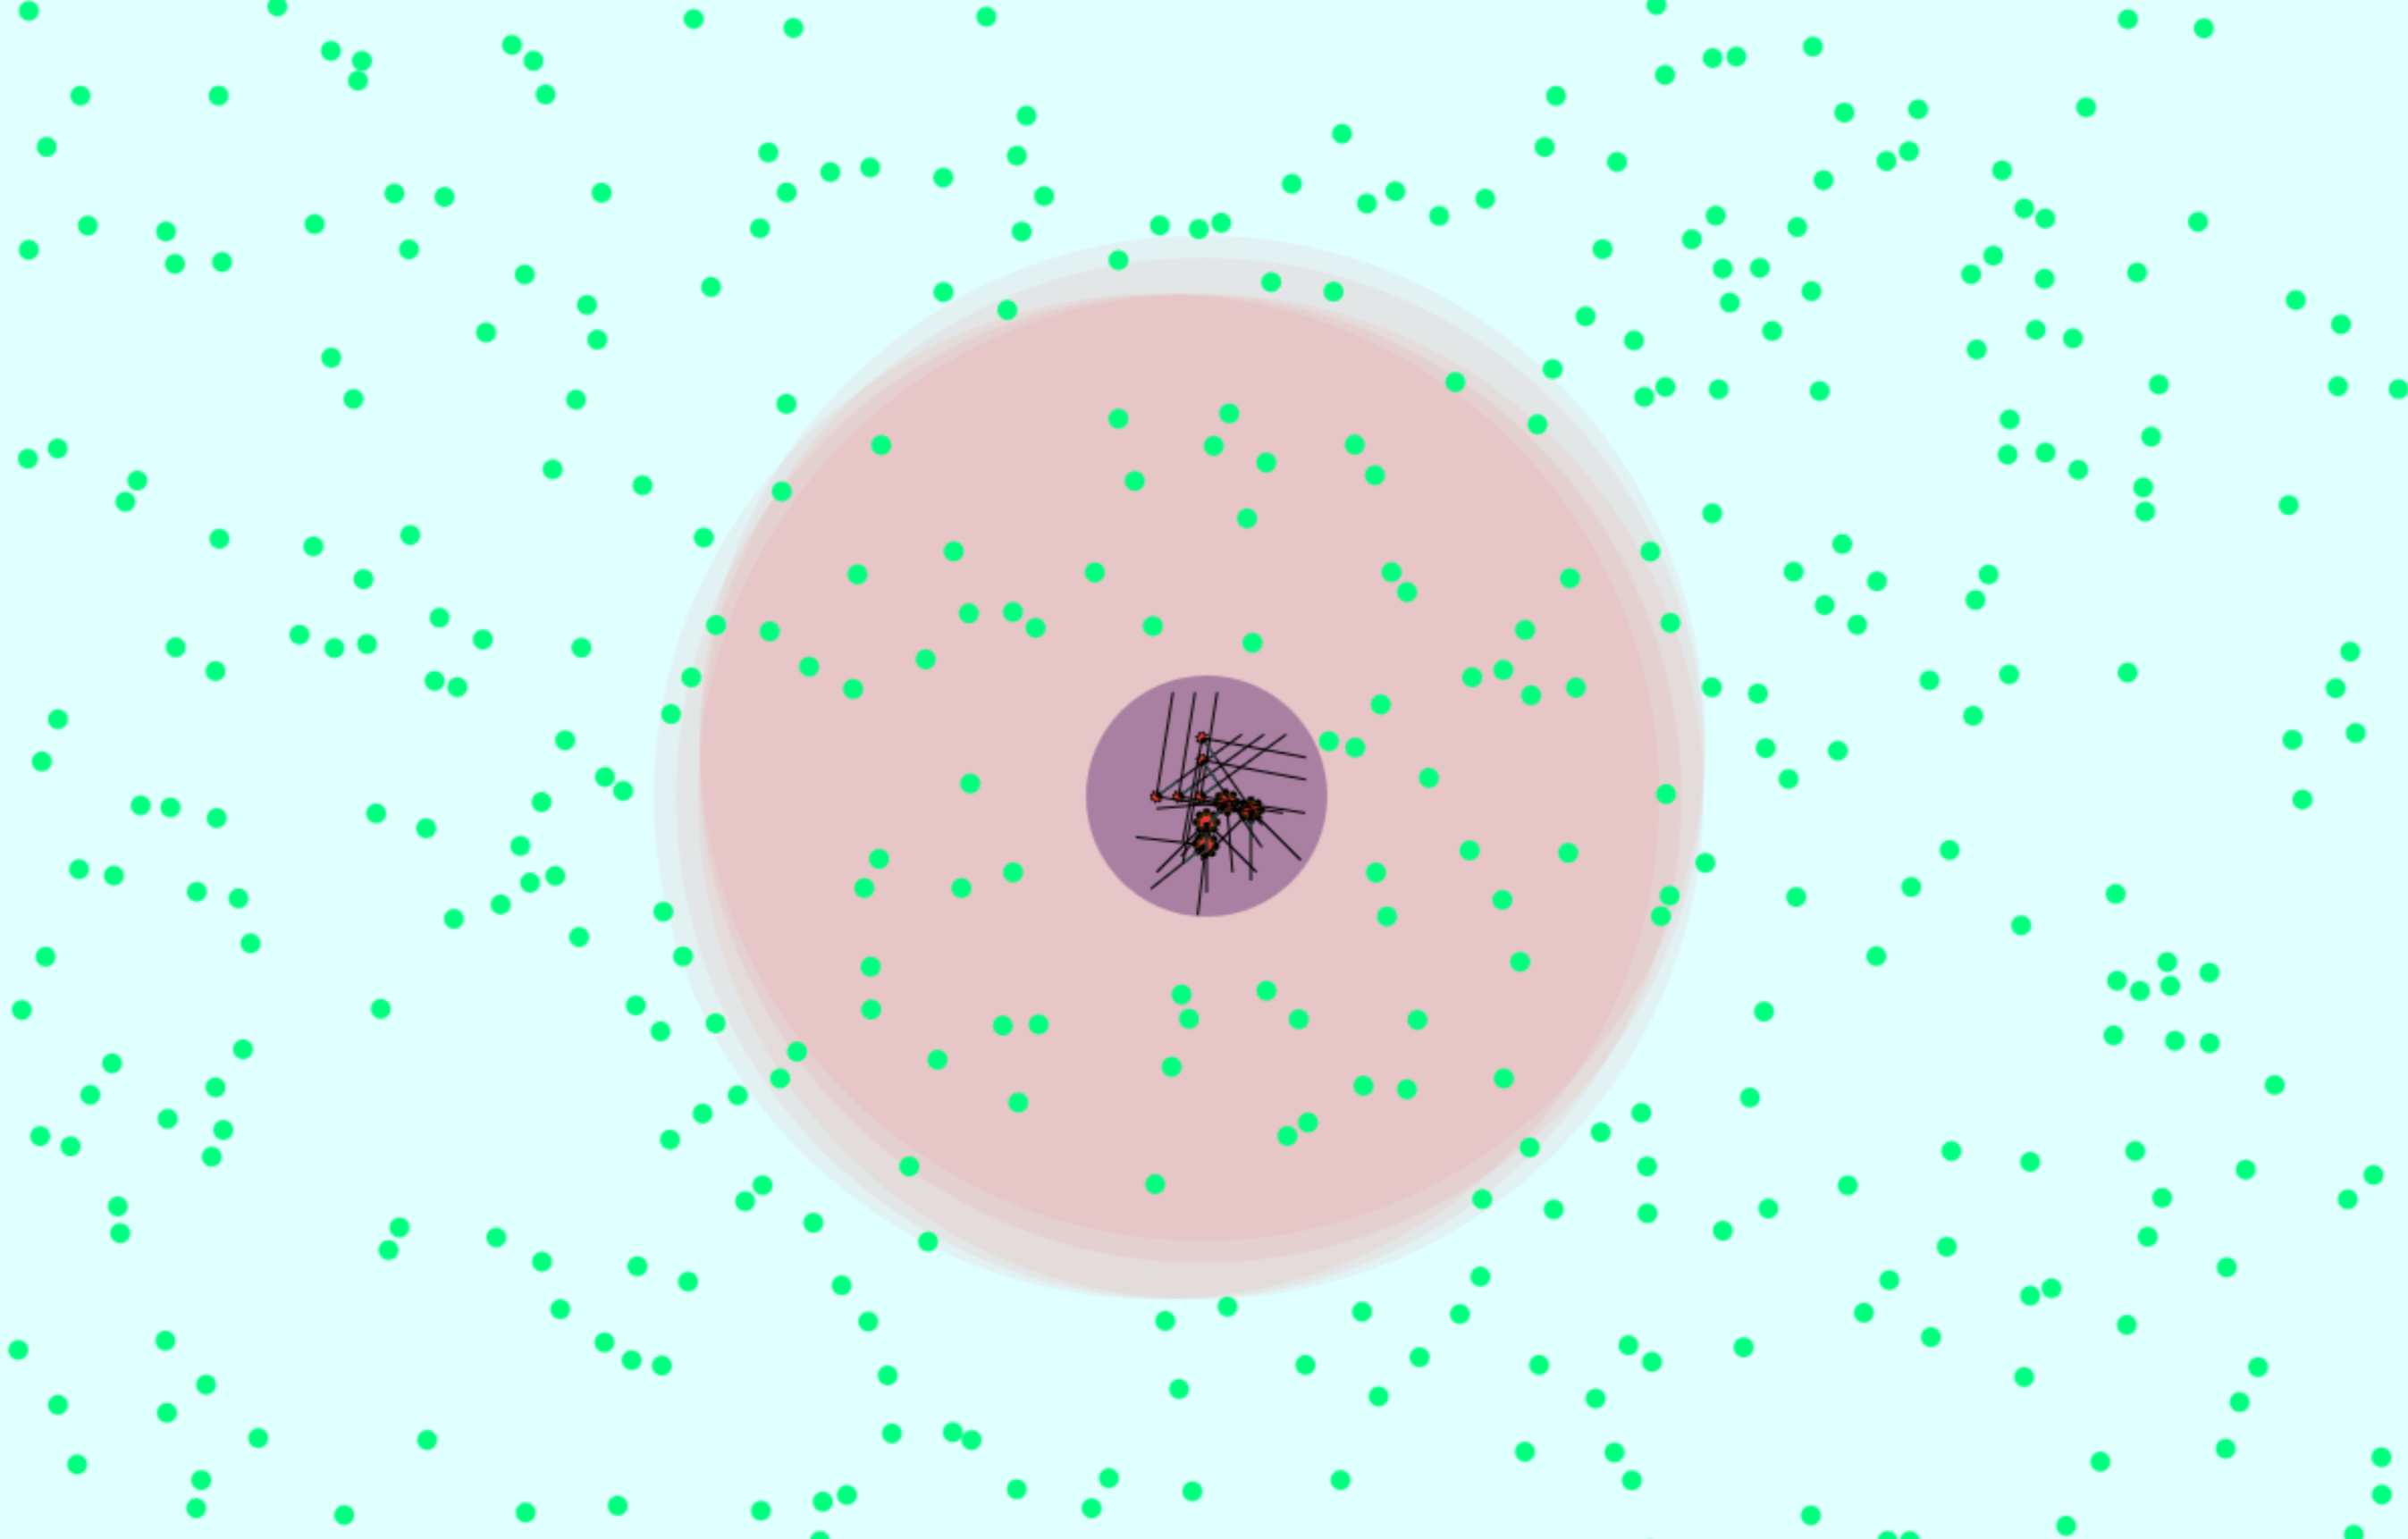
\includegraphics[width=\columnwidth]{../img/WoodMap/pictures/StartRandom.png}
	\caption{Příklad WoodScene mapy: start náhodného chování}
	\label{obr04:WoodSceneRandomStart}
\end{figure}
\par

\begin{figure}[p]\centering
	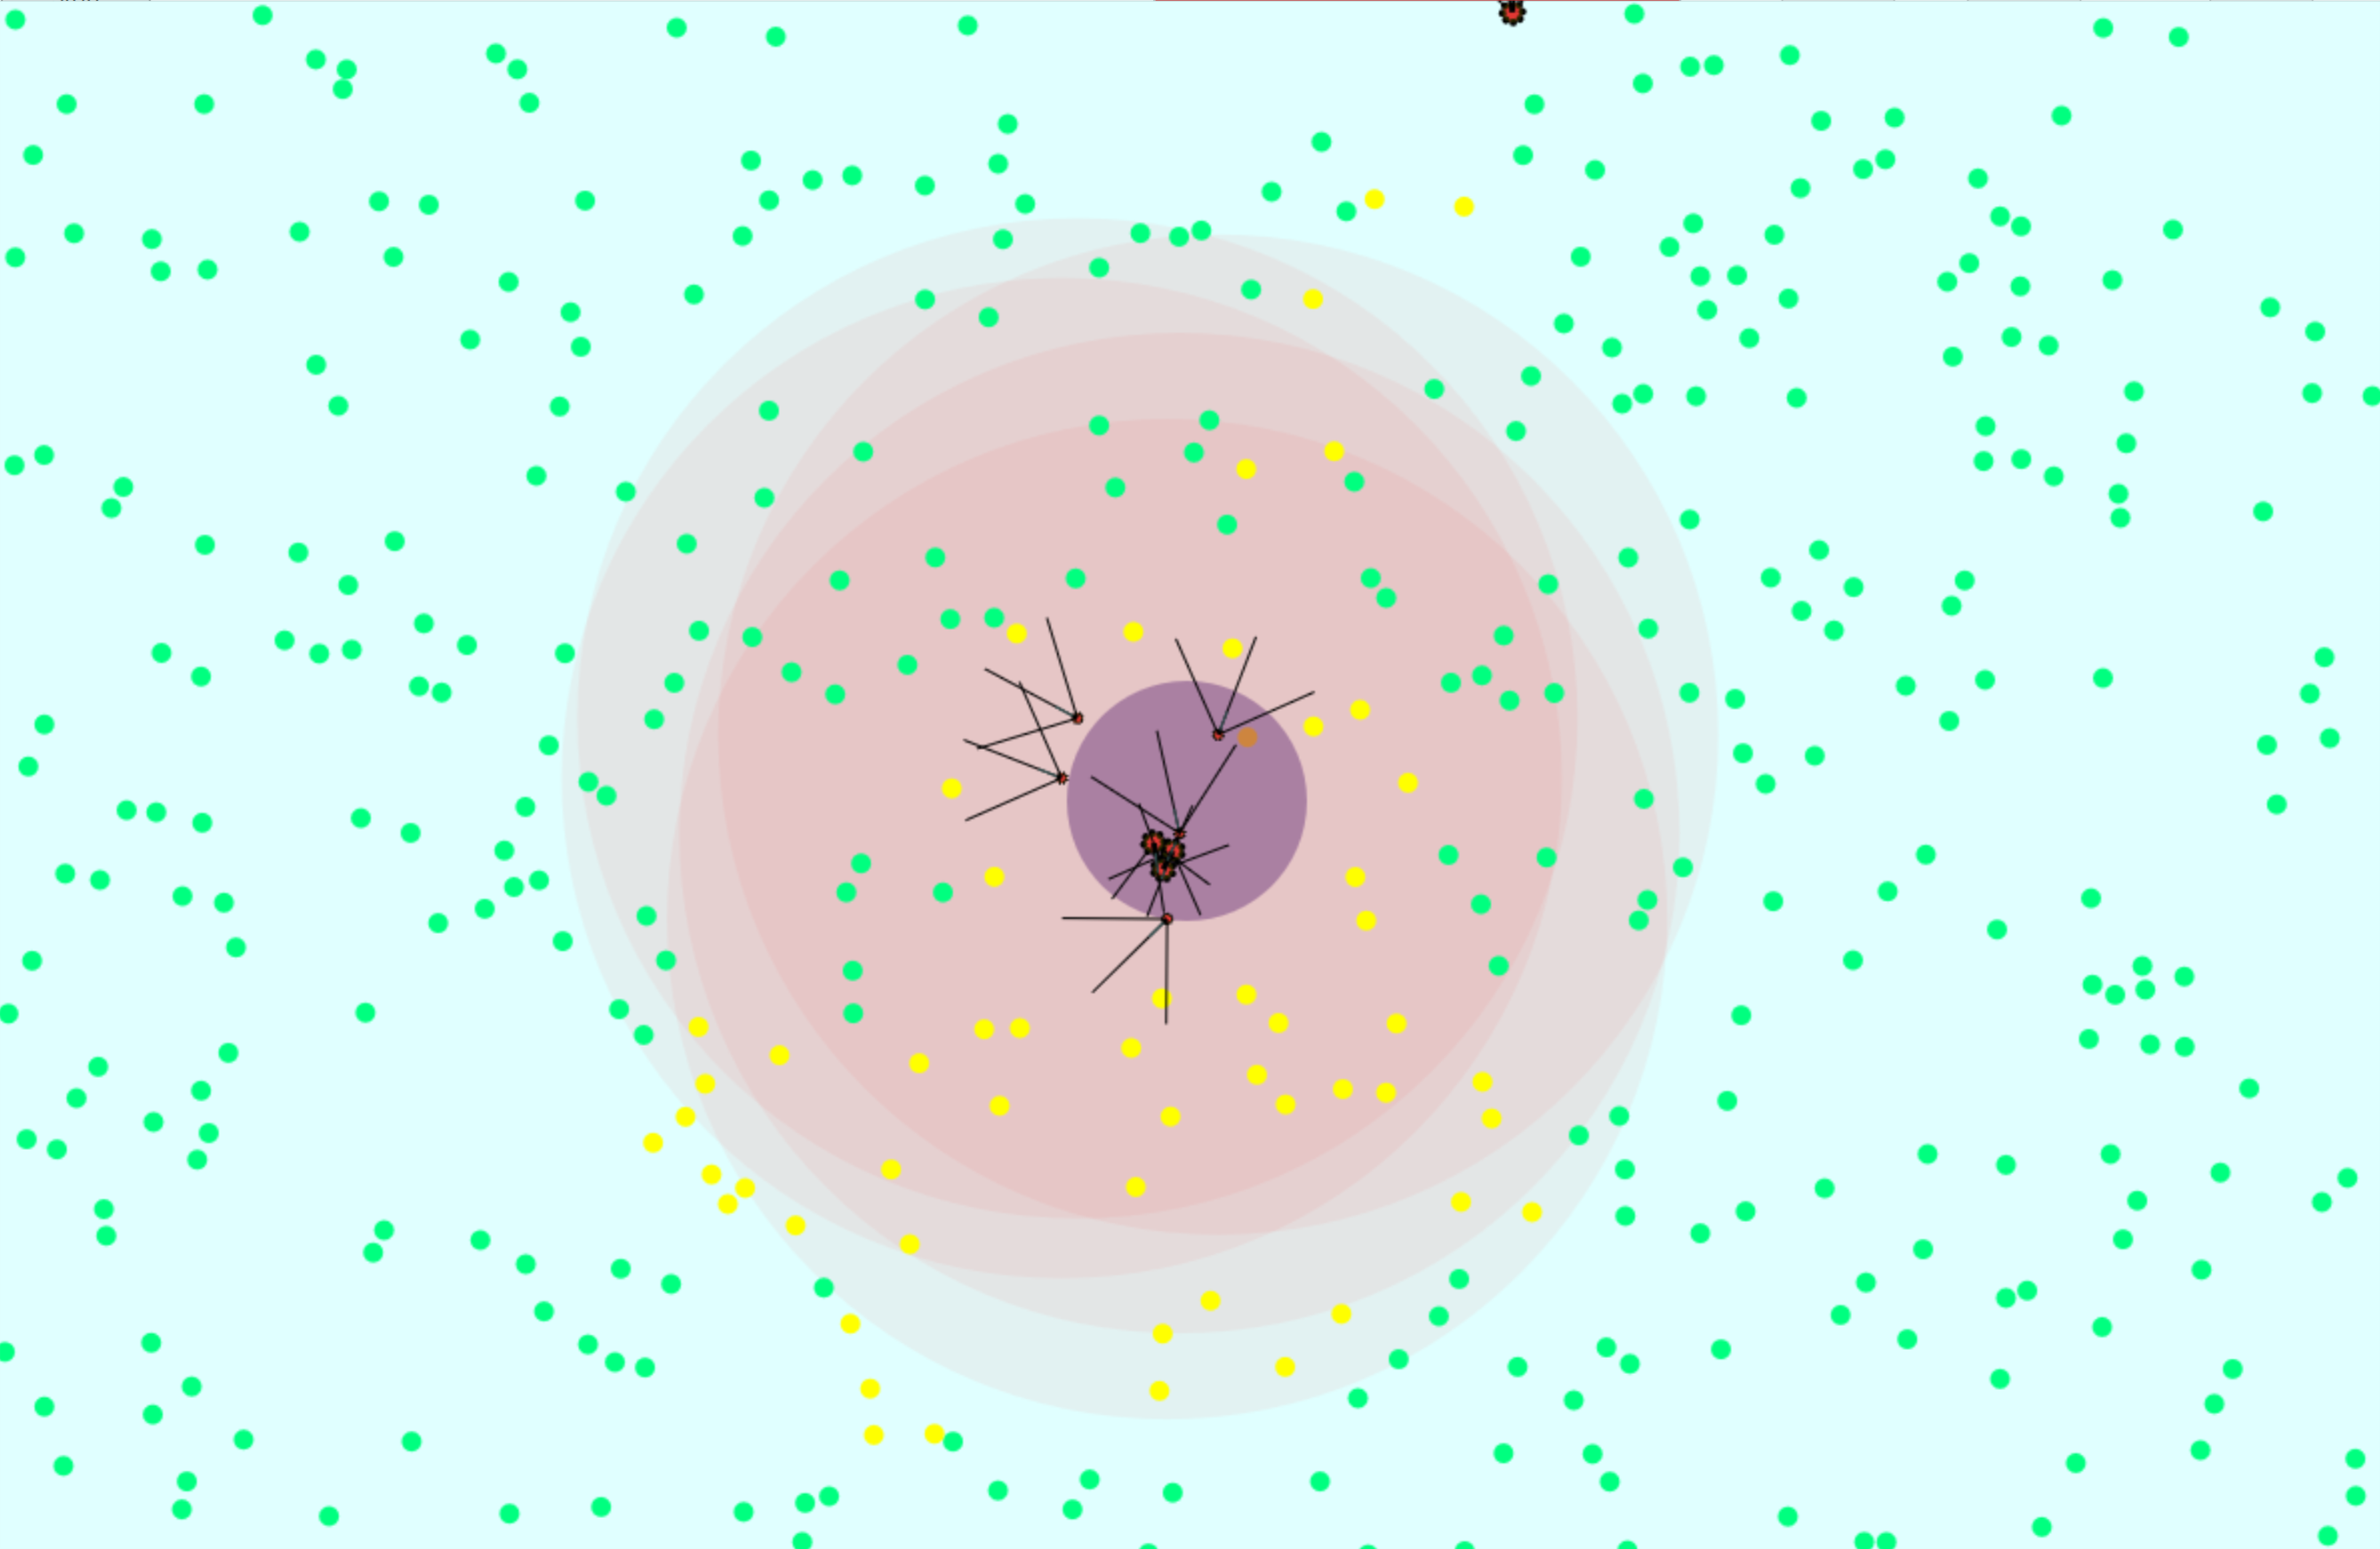
\includegraphics[width=\columnwidth]{../img/WoodMap/pictures/EndRandom.png}
	\caption{Příklad WoodScene mapy: po 9000 iteracích náhodného chování}
	\label{obr04:WoodSceneRandomEnd}
\end{figure}
\clearpage
\subsection{Roboti}
\subsubsection{Scout robot}
Jedná se o robota, který má na starosti průzkum mapy a kácení nalezených stromů. Pro komunikaci s ostatními roboty má možnost vysílat rádiový signál s hodnotou 0. Oproti Worker robotovi je menší, rychlejší, jeho senzory mají větší dosah, navíc proti němu disponuje type senzorem a refaktorem nalezených stromů. Type senzor představuje formu radaru, říká robotovi s jakou četností se vyskytují v dosahu senzoru. Refaktor reprezentuje techniku kácení mění strom na dřevo. 
\par 
\begin{center}
\begin{tabular}{l@{\hspace{1.0cm}}D{.}{,}{2.2}D{.}{,}{2.2}D{.}{,}{2.3}}
	\toprule
	\mc{Scout Robot} \\
	\midrule
        Tvar: & Kruh & \\
        Poloměr: & 2.5 \\
        Název: & WoodCutterM \\
        Velikost kontejner: & 0\\
        \hline
        Efektory \\
        \midrule
        Motor: & Dvou kolečkový \\
        Maximální rychlost: & 3 \\
        Kód rádiového signálu: & 0 \\
        Poloměr signálu: & 200\\
        Refaktor: & Strom \Rightarrow Dřevo \\
        Dosah refaktoru: & 10\\
        Počet paměťových slotů: & 10 \\
        Obsah slotu: & float\\
        \hline 
        Senzory \\
        \midrule
        Počet line senzorů: &  3 \\
        Délka line senzorů: & 50\\
        Orientace line senzorů: & 0^\circ, 45^\circ, -45^\circ \\
        Poloměr type senzoru: & 50\\
        Poloměr rádiového přijímače: &  100 \\
        Počet touch senzorů: & 8 \\  
        Lokátor senzor\\ 
	\bottomrule
	\multicolumn{2}{l}{\footnotesize \textit{Pozn:}
	Scout robot popis}
\end{tabular}
\end{center}
\subsubsection{Worker robot}
Worker robot se stará o transport objektů na mapě. Ke komunikaci využívá signálů s kódem 1. Sebrané objekty ukládá do kontejneru, kam se vejde 5 entit. Zvedání a pokládání probíhá skrze efektor Picker. 
\par 
\begin{center}
	\begin{tabular}{l@{\hspace{1.0cm}}D{.}{,}{2.2}D{.}{,}{2.2}D{.}{,}{2.3}}
			\toprule
			\mc{Worker Robot} \\
			\midrule
                Tvar: & Kruh\\
                Poloměr: & 5\\
                Název: & WoodWorkerM \\
                Velikost kontejner: & 5\\
                \hline
                Efektory \\
                \midrule
                Motor: & Dvou kolečkový \\
                Maximální rychlost: & 2 \\
                Kód rádiového signálu: & 0\\
                Poloměr signálu: & 200\\
                Dosah pickeru: & 10\\
                Počet paměťových slotů: &10 \\
                Obsah slotu: & float\\
                \hline 
                Senzory \\
                \midrule
                Počet line senzorů: &  3\\
                Délka line senzorů: & 30\\
                Orientace line senzorů: & 0^\circ, 45^\circ, -45^\circ\\
                Poloměr rádiového přijímače: & 100 \\
                Počet touch senzorů: & 8 \\  
                Lokátorový senzor\\ 
	\bottomrule
\multicolumn{2}{l}{\footnotesize \textit{Pozn:}
	Scout robot popis}
\end{tabular}
\end{center}
\subsection{Vyhodnocování Fitness}
Fitness funkce pro ohodnocení WoodScene scénáře probíhá vždy až na konci simulace. I když se úspěšnost v pod-úkolech  vždy posuzuje jinak, celou fitness funkci lze shrnout do následujícího cílů. Roboti jsou odměňováni za: 
\begin{enumerate}
        \item kolize = počet pokusů o pohyb při kterém by došlo ke kolizi 
        \item nalezené stromy = stromy o které zavadil line senzor 
        \item pokácené stromy = stromy, které refaktor změnil 
        \item sebrané dřevo = zpracované dřevo, které mají roboti uvnitř kontejnerů 
        \item uskladněné dřevo = dřevo, které dovezli na vyznačené místo 
\end{enumerate}

\subsection{Pod-úkoly} 
Pro oba použité algoritmy jsem používal stejné úlohy pro naučení robotů postupně těžších a těžších cílů. Hlavně také, abych mohl porovnat oba evoluční algoritmy.  
\begin{enumerate}
        \item vygenerování robotů = Na začátku je vygenerováno chování robotů naprosto náhodně. Pro každého robota, je vygenerována náhodná jednovrstvá neuronová síť. 
        \item učení chůze = Pro oba roboty je velmi důležité, aby se pohybovali bez kolizí po celé mapě a objevovali, co největší prostor. Roboti jsou vyvíjeni odděleně a fitness se soustředí na počet kolizí(záporným ohodnocením) a na nalezené stromy(kladným ohodnocením).
        \item těžba stromů = Scout roboty, kteří se už obstojně po mapě pohybují, je třeba naučit kácet stromy. Proto dalším pod-úkol cílí ve fitness funkci na počet pokácených stromů. Nicméně stále také na počet stromů nalezených. 
        \item převoz dřeva = Správně pohybující chceme naučit sbírat vytěžené dřevo. Fitness hodnotí počet sebraného dřeva, případně i uskladněné dřevo. Na těchto mapách jsou už na začátku připraveny pouze entity zpracovaného dřeva.
        \item kooperace = V posledním experimentu, se hodnotí pouze sebrané a uskladněné dřevo. A evolvují se oba druhy robotů současně. 
\end{enumerate}
\begin{center}
	\subsubsection{Nastavení parametrů}
	\begin{tabular}{l@{\hspace{1.5cm}}D{.}{,}{3.2}D{.}{,}{1.2}D{.}{,}{2.3}}
		\toprule
		& \mc{} & \mc{}\\
		\pulrad{\textbf{Parametr:}} & \mc{\pulrad{\textbf{Hodnota:}}}\\
		\midrule
		F(DE):     & 0.8 \\
		CR(DE):  & 0.5 \\
		alpha(ES) & 0.05 \\
		sigma(ES) & 0.1\\
		\bottomrule
		\multicolumn{2}{l}{\footnotesize \textit{Pozn:}
			Nastavení evolučních algoritmů}
	\end{tabular}
	\par 
\end{center}
\newpage
	\subsubsection{Scout chůze - nastavení experimentu}
	\begin{table}[h]\centering
		\begin{tabular}{l@{\hspace{1.5cm}}D{.}{,}{3.2}D{.}{,}{1.2}D{.}{,}{2.3}}
			\toprule
			& \mc{} & \mc{}\\
			\pulrad{\textbf{Vlastnost:}} & \mc{\pulrad{\textbf{Hodnota:}}}\\
			\midrule
			Roboti:     & Scout-5 \\
			Počet generací: & 1000\\
			Počet iterací map & 1000\\
			Velikost generace(DE) & 200\\
			Počet jedinců(ES) & 10\\
			Počet mutovaný potomků(ES)&20\\
			Elitismus(ES)& Ano\\
			Elitismus(DE)& Ne \\
			\bottomrule
			\multicolumn{2}{l}{\footnotesize \textit{Pozn:}
			Nastavení evolučních algoritmů}
		\end{tabular}
		\begin{tabular}{l@{\hspace{1.5cm}}D{.}{,}{3.2}D{.}{,}{1.2}D{.}{,}{2.3}}
			\toprule
			& \mc{} & \mc{}\\
			\pulrad{\textbf{Vlastnost:}} & \mc{\pulrad{\textbf{Hodnota:}}}\\
			\midrule
			Hodnota nalezeného stromu &  10 \\
			Ostatní hodnoty: & 0\\
			Počet stromů: & 300\\
			Počet už pokácených stromů & 100\\
			\bottomrule
			\multicolumn{2}{l}{\footnotesize \textit{Pozn:}
				Nastavení hodnocení fitness}
		\end{tabular}
	\caption{Scout chůze - nastavení experimentu}\label{tab04:ScoutWalk}
	\end{table}
	
	\begin{figure}[t]\centering
		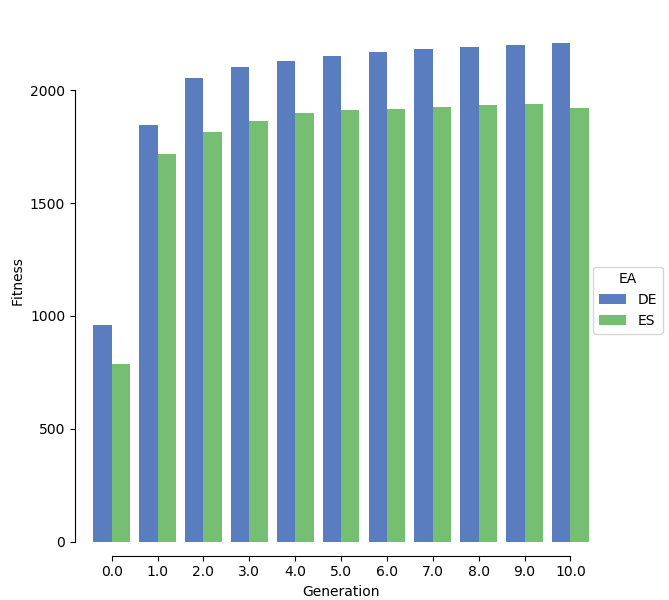
\includegraphics[width=\columnwidth]{../img/WoodMap/DEvsES/WCuttorWalkMem.png}
		\caption{ Scout chůze - porovnání průměrné fitness ES a DE}
		\label{obr04:WalkESvsDE}
	\end{figure}
	\redo{Opravit obrázky - rozsahy a popisy}
	\begin{figure}[p]
		\centering
		\begin{subfigure}{.5\textwidth}
			\centering
			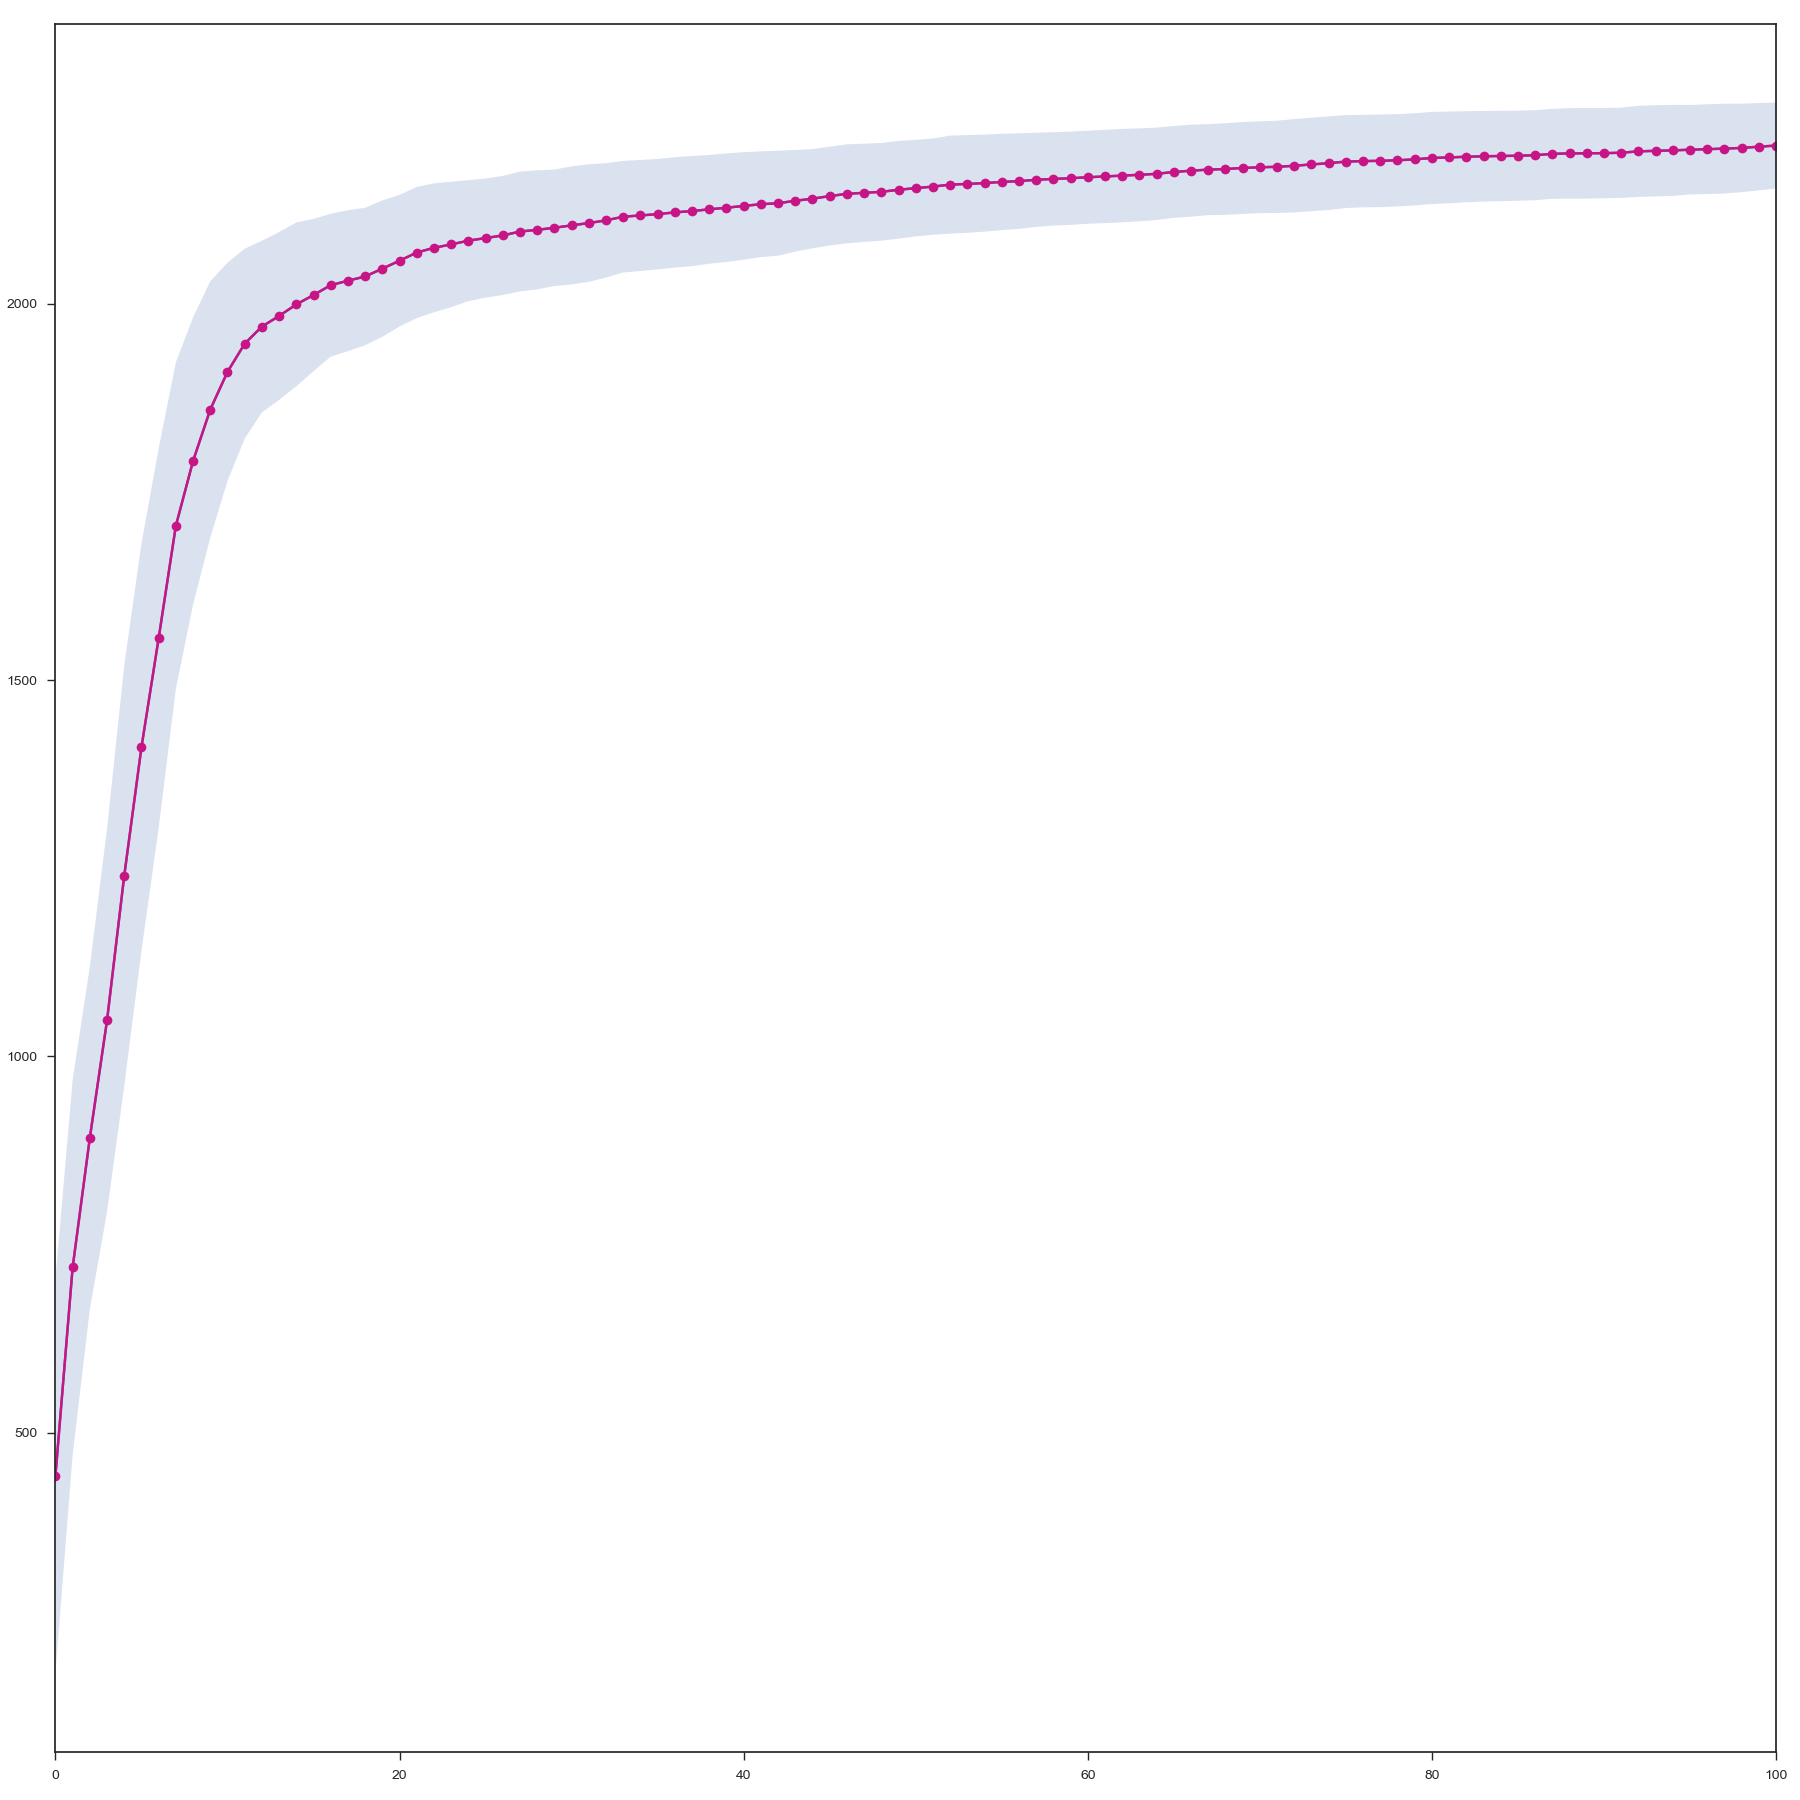
\includegraphics[width=\linewidth]{../img/WoodMap/DE/graph_of_CuttorWalk-mean.png}
			\caption{DE}
			\label{obr04:WalkDE}
		\end{subfigure}%
		\begin{subfigure}{.5\textwidth}
			\centering
			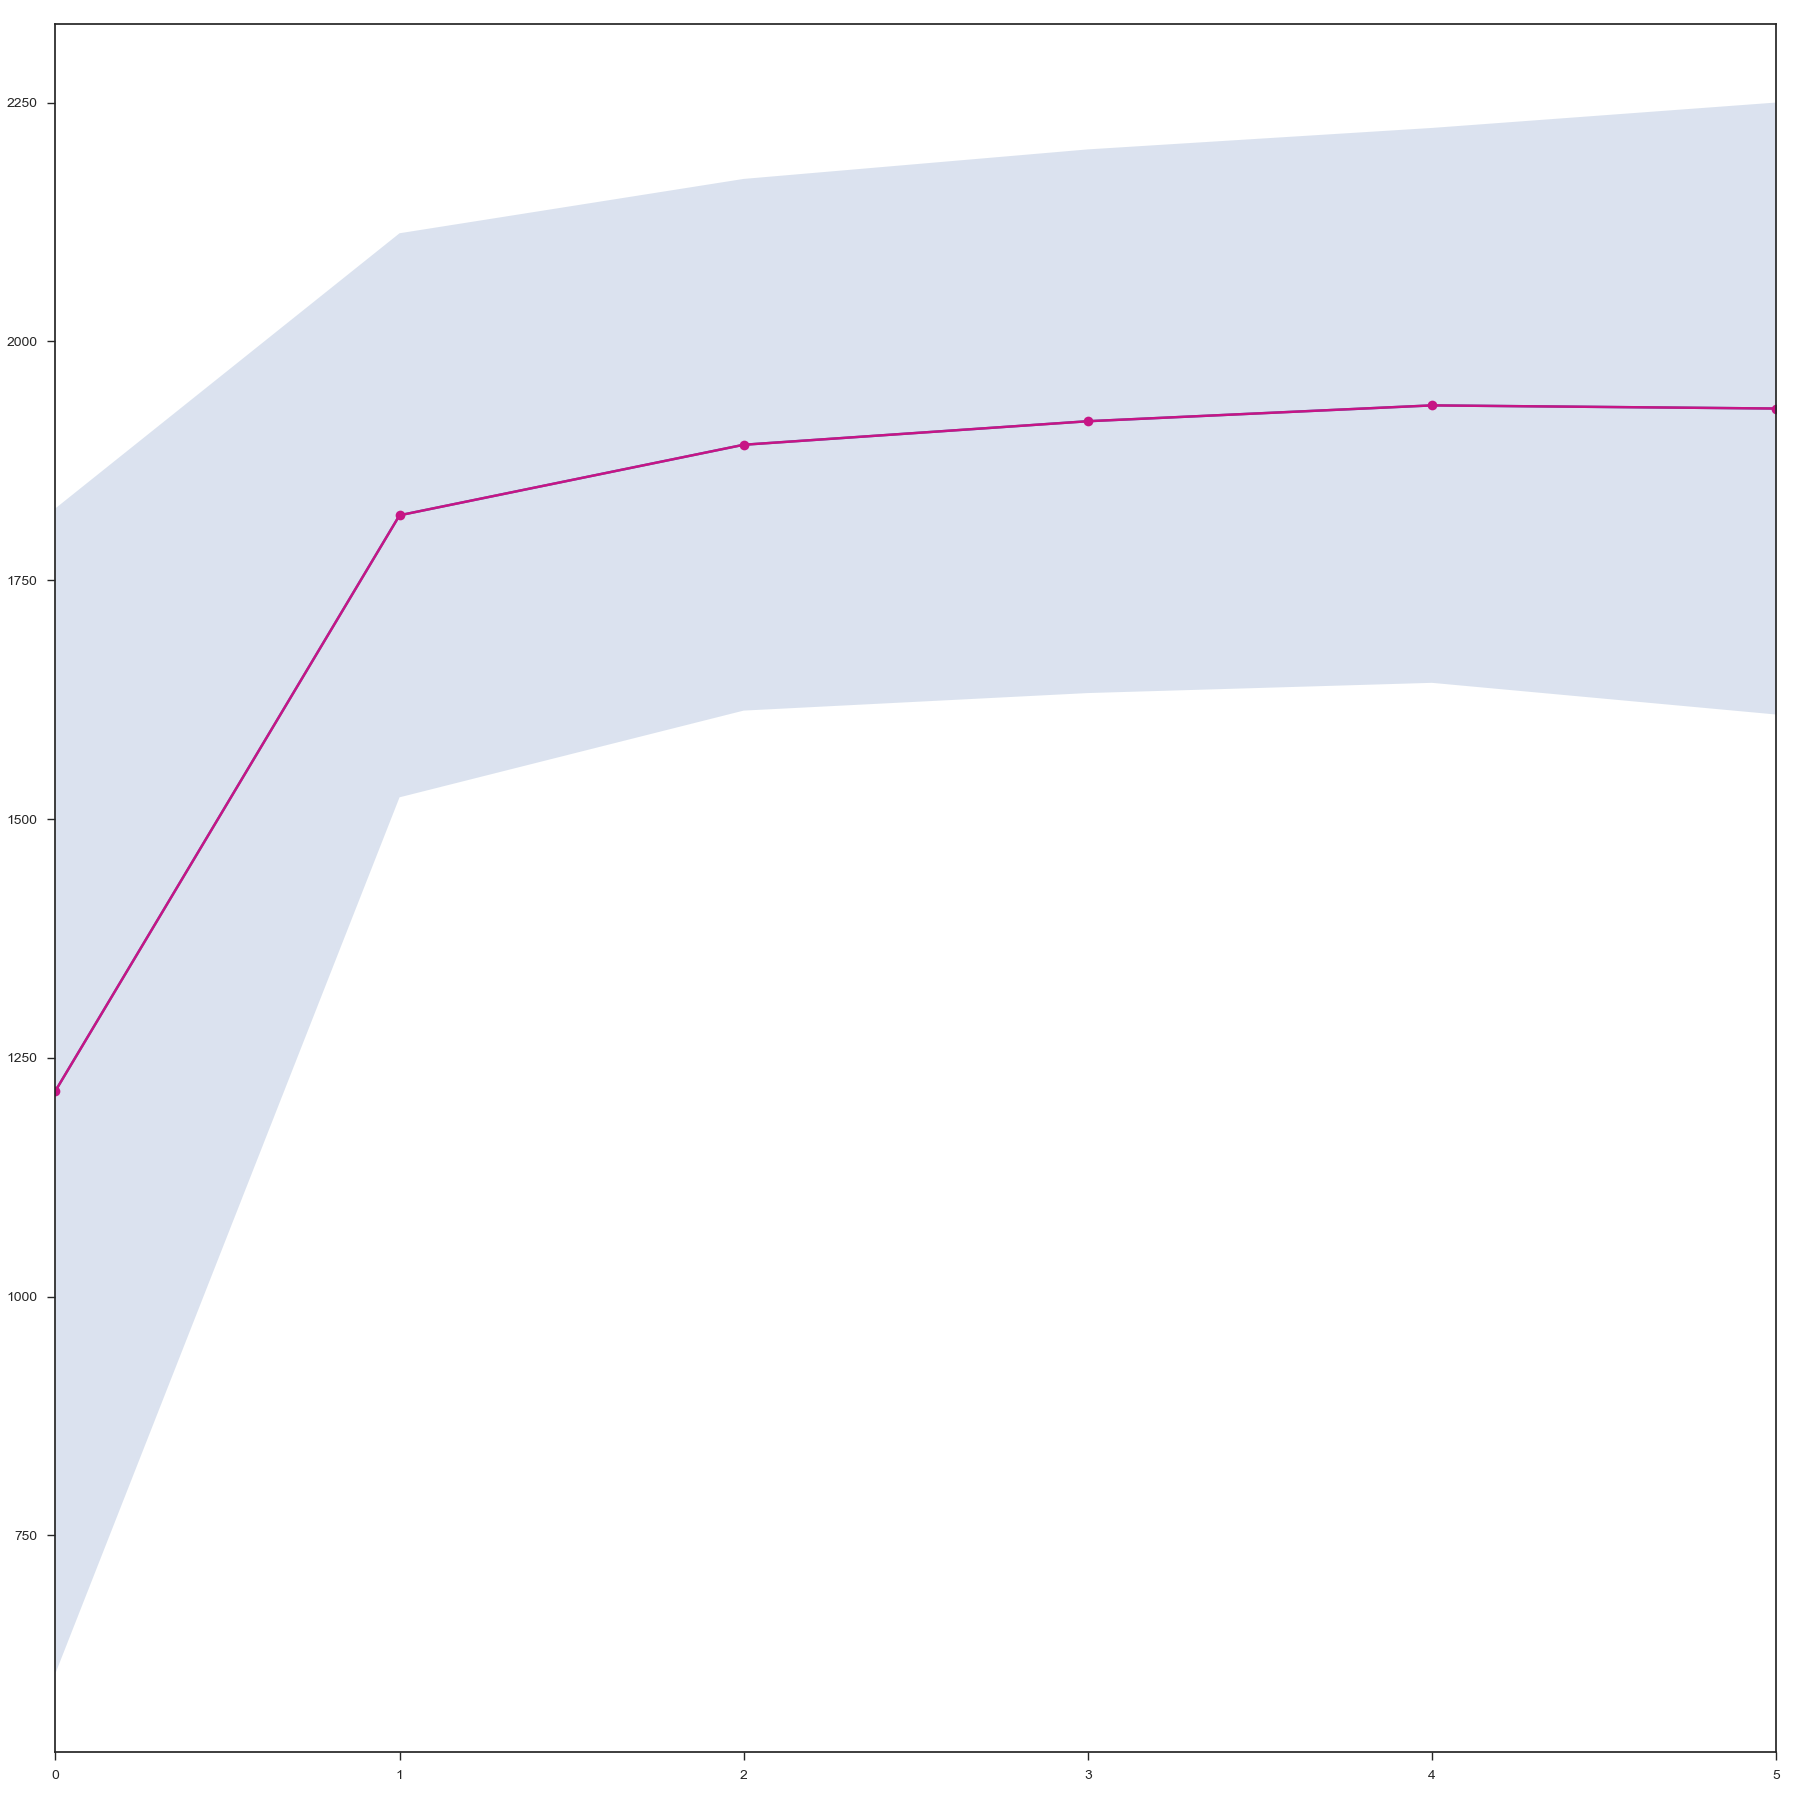
\includegraphics[width=\linewidth]{../img/WoodMap/ES/WoodWalkES-mean.png}
			\caption{ES}
			\label{obr04:WalkES}
		\end{subfigure}
		\caption{Scout chůze - průběh fitness }
		\label{obr04:Walk}
	\end{figure}
	\clearpage
  
	\subsubsection{Worker chůze - nastavení experimentu}
	\begin{table}[h]\centering
		\begin{tabular}{l@{\hspace{1.5cm}}D{.}{,}{3.2}D{.}{,}{1.2}D{.}{,}{2.3}}
			\toprule
			& \mc{} & \mc{}\\
			\pulrad{\textbf{Vlastnost:}} & \mc{\pulrad{\textbf{Hodnota:}}}\\
			\midrule
			Roboti:     & Worker-4 \\
			Počet generací: & 1000\\
			Počet iterací map & 1000\\
			Velikost generace(DE) & 200\\
			Počet jedinců(ES) & 10\\
			Počet mutovaný potomků(ES)&20\\
			Elitismus(ES)& Ano\\
			Elitismus(DE)& Ne \\
			\bottomrule
			\multicolumn{2}{l}{\footnotesize \textit{Pozn:}
				Nastavení evolučních algoritmů}
		\end{tabular}
		\begin{tabular}{l@{\hspace{1.5cm}}D{.}{,}{3.2}D{.}{,}{1.2}D{.}{,}{2.3}}
			\toprule
			& \mc{} & \mc{}\\
			\pulrad{\textbf{Vlastnost:}} & \mc{\pulrad{\textbf{Hodnota:}}}\\
			\midrule
			Hodnota nalezeného pokáceného stromu &  100 \\
			Ostatní hodnoty: & 0\\
			Počet stromů: & 200\\
			Počet už pokácených stromů & 200\\
			\bottomrule
			\multicolumn{2}{l}{\footnotesize \textit{Pozn:}
				Nastavení hodnocení fitness}
		\end{tabular}
		\caption{Worker chůze - nastavení experimentu}
		\label{tab04:WorkerWalk}
	\end{table}

	\begin{figure}[t]\centering
		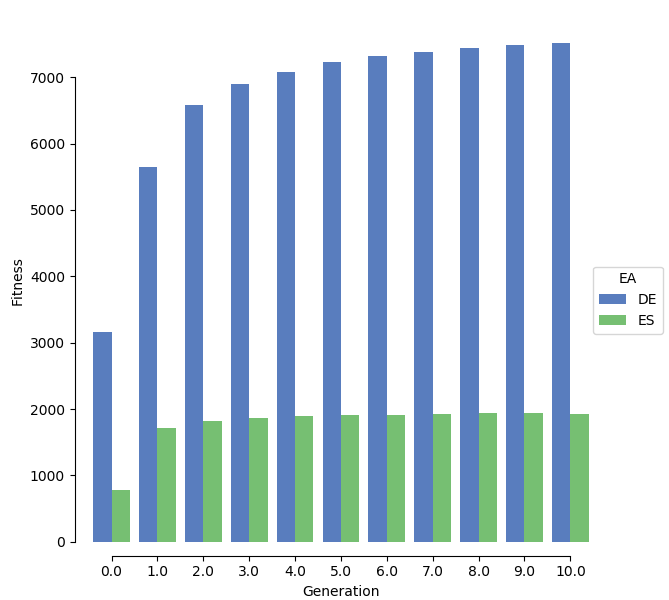
\includegraphics[width=\columnwidth]{../img/WoodMap/DEvsES/WorkerWalkMem.png}
		\caption{Worker chůze - porovnání průměrné fitness ES a DE}
		\label{obr04:WWalkESvsDE}
	\end{figure}
	\redo{Opravit rozsahy a rozlišení}
	\begin{figure}[p]
		\centering
		\begin{subfigure}{.5\textwidth}
			\centering
			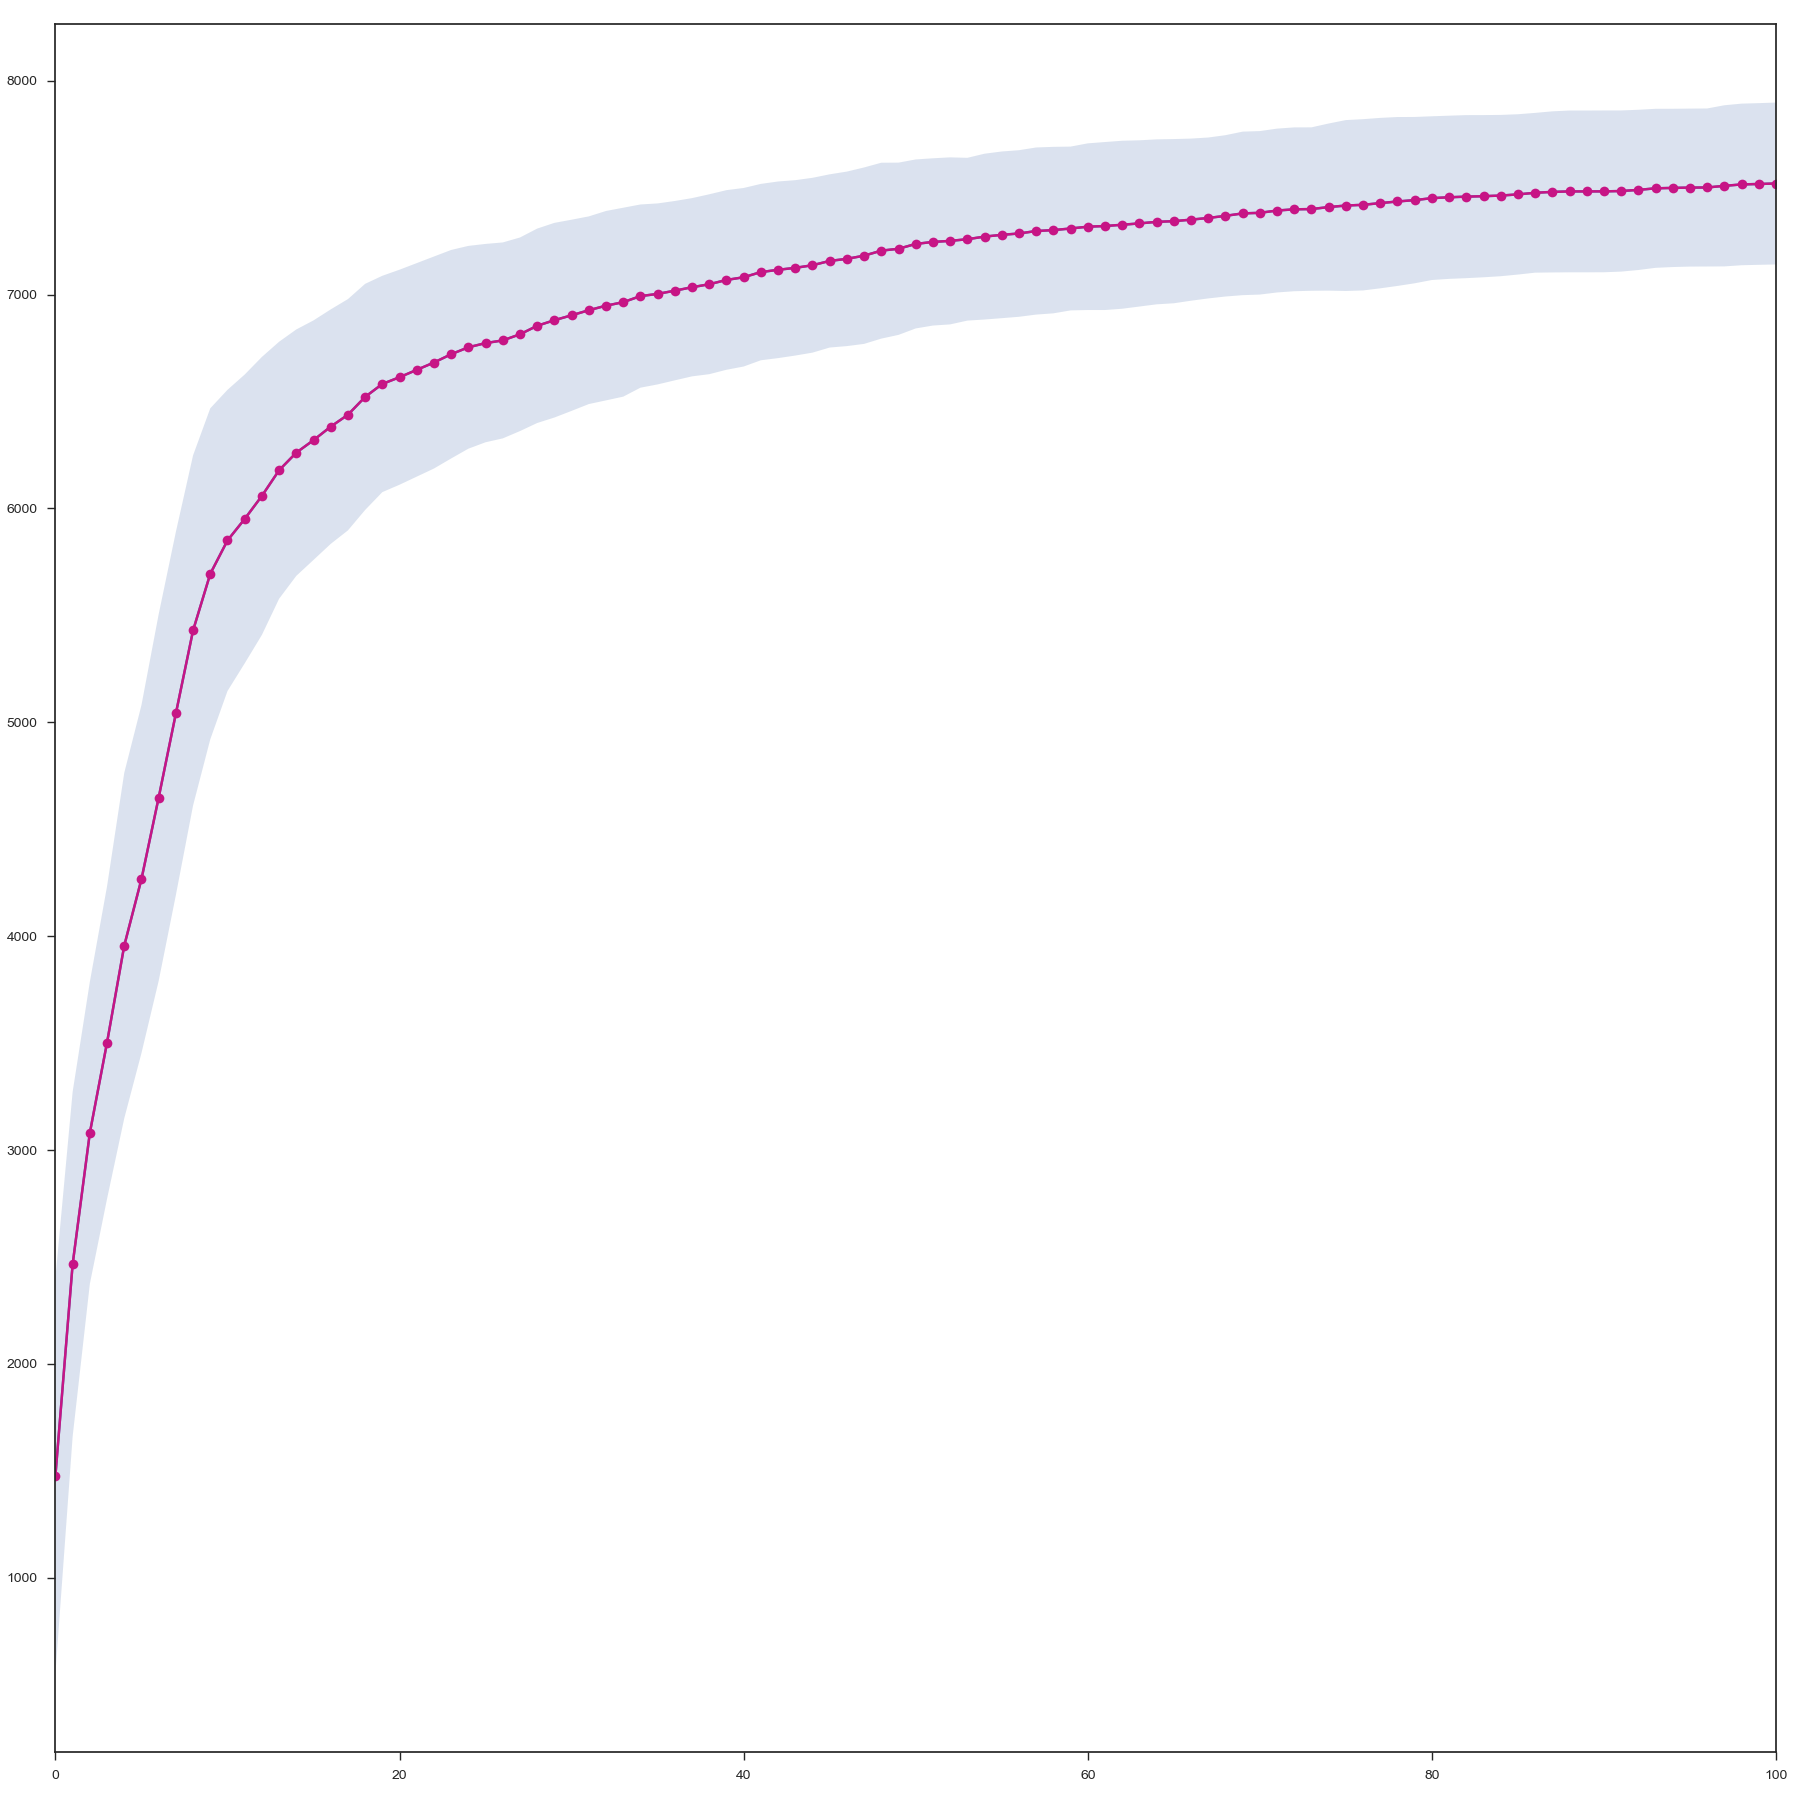
\includegraphics[width=\linewidth]{../img/WoodMap/DE/graph_of_WorkerWalkMem-mean.png}
			\caption{DE}
			\label{obr04:WWalkDE}
		\end{subfigure}%
		\begin{subfigure}{.5\textwidth}
			\centering
			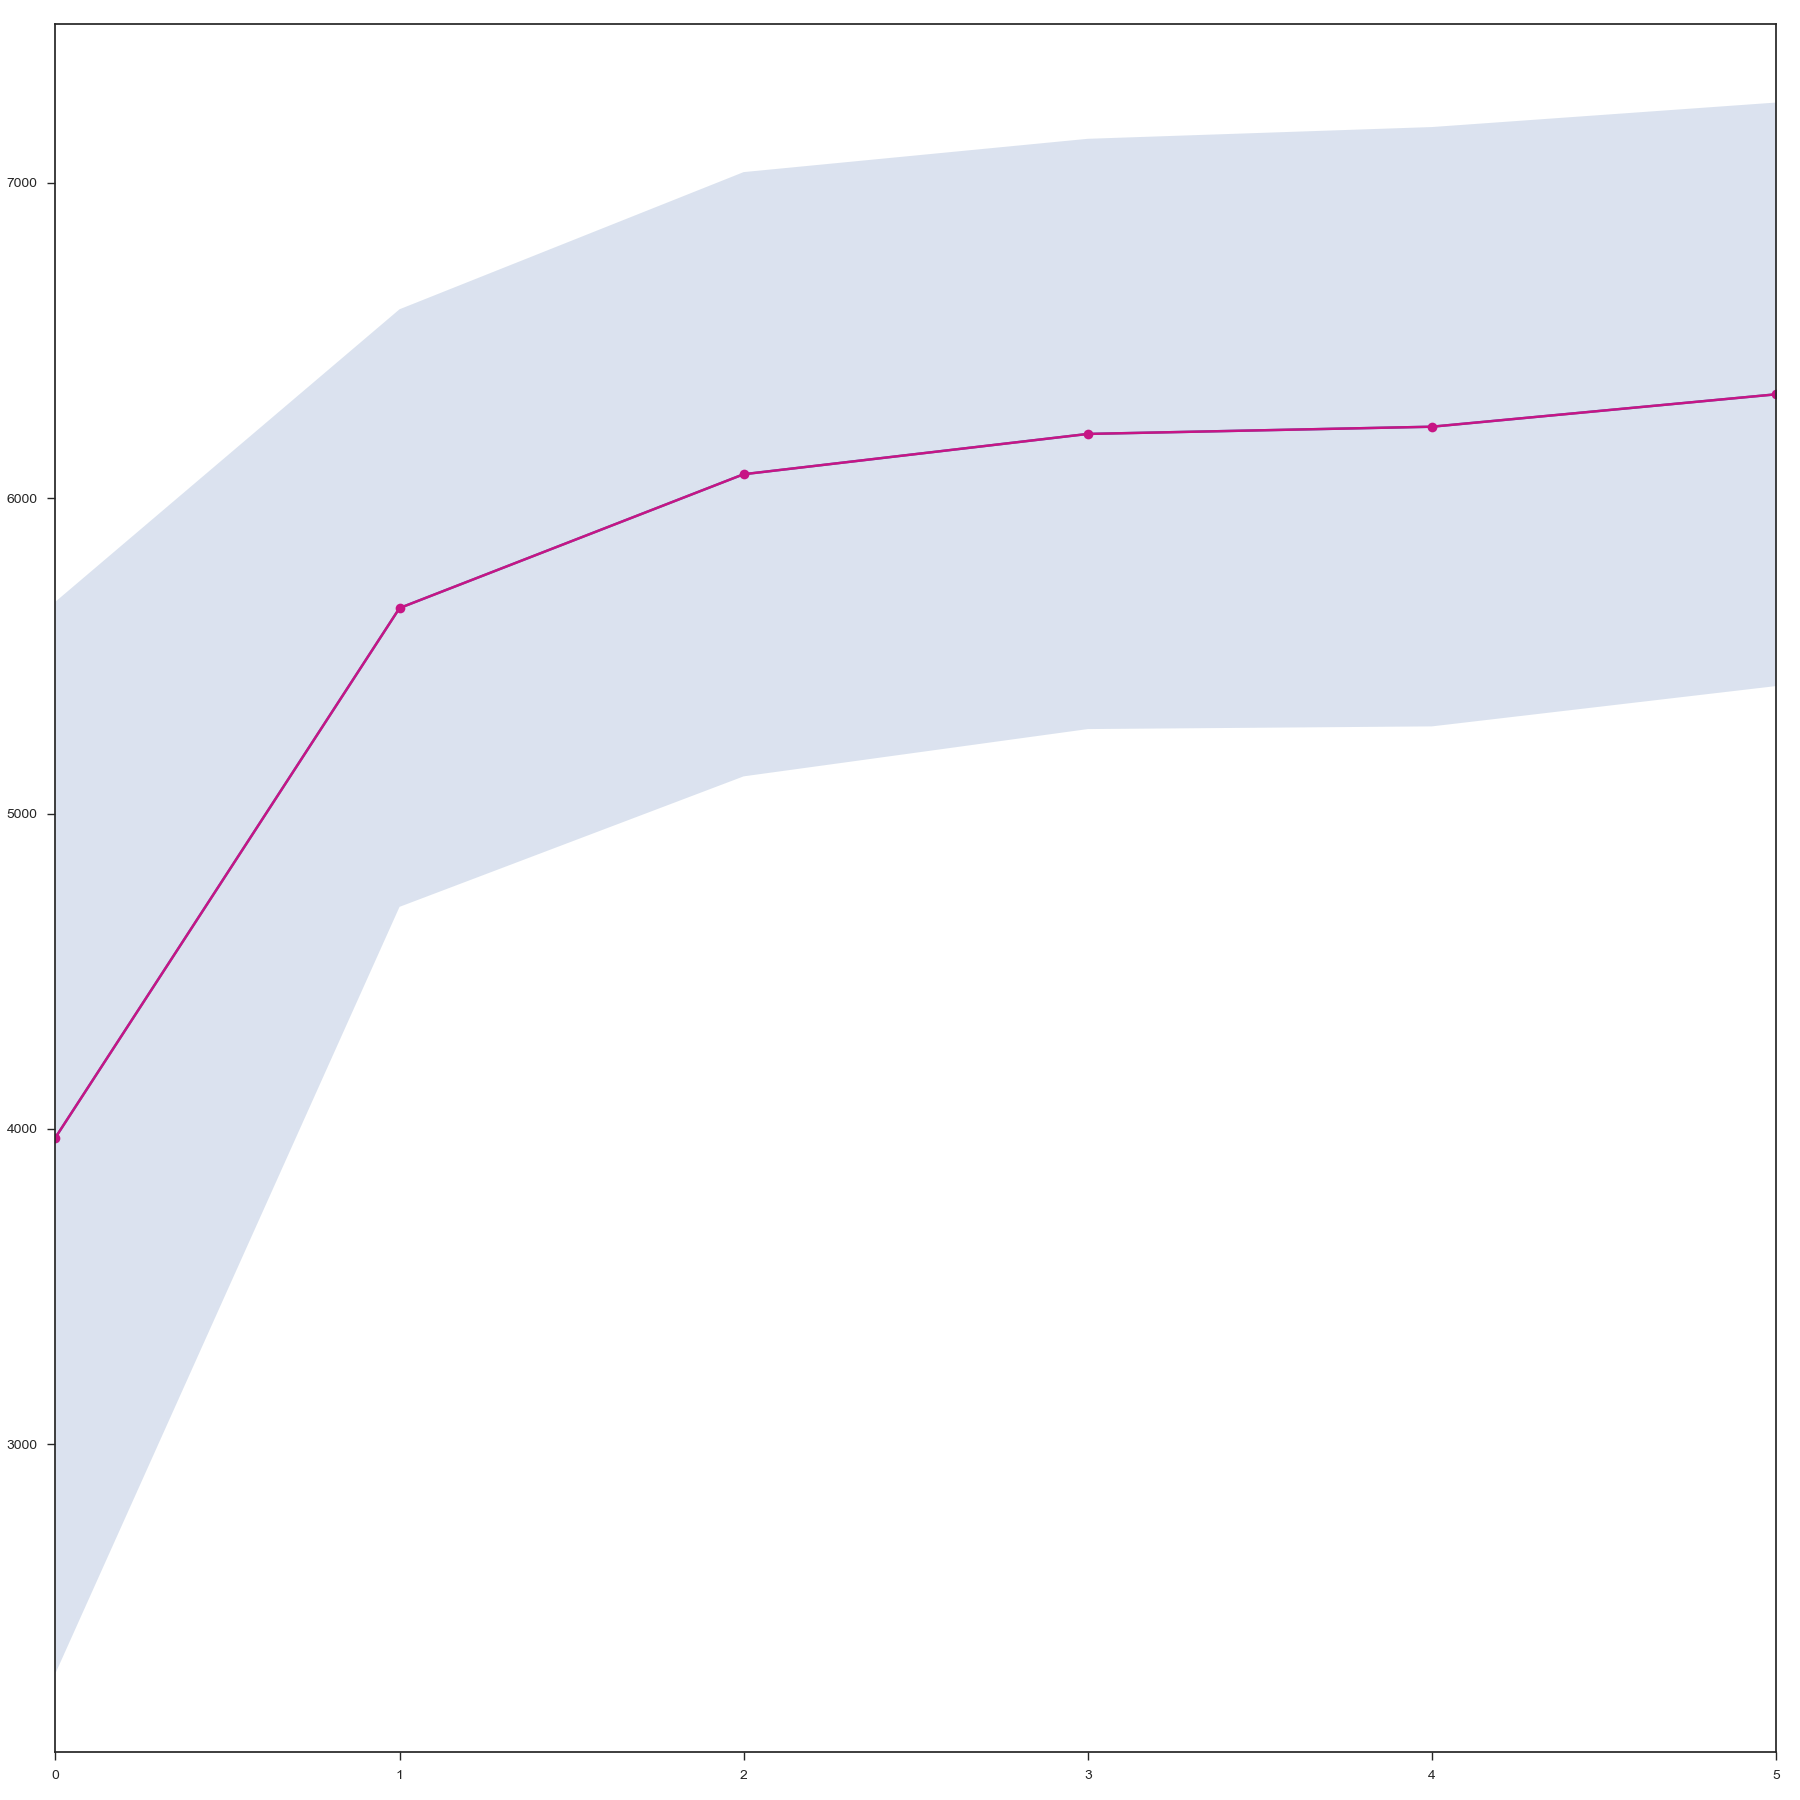
\includegraphics[width=\linewidth]{../img/WoodMap/ES/WoodWWalkES-mean.png}
			\caption{ES}
			\label{obr04:WWalkES}
		\end{subfigure}
		\caption{Worker chůze - průběh fitness v rámci generací}
		\label{obr04:WWalk}
	\end{figure}
	\clearpage 
	
	

	\subsubsection{Scout kácení - nastavení experimentu}
		\begin{table}[h]\centering
		\begin{tabular}{l@{\hspace{1.5cm}}D{.}{,}{3.2}D{.}{,}{1.2}D{.}{,}{2.3}}
			\toprule
			& \mc{} & \mc{}\\
			\pulrad{\textbf{Vlastnost:}} & \mc{\pulrad{\textbf{Hodnota:}}}\\
			\midrule
			Roboti:     & Scout-5 \\
			Počet generací: & 1500\\
			Počet iterací map & 1000\\
			Velikost generace(DE) & 200\\
			Počet jedinců(ES) & 10\\
			Počet mutovaný potomků(ES)&20\\
			Elitismus(ES)& Ano\\
			Elitismus(DE)& Ne \\
			\bottomrule
			\multicolumn{2}{l}{\footnotesize \textit{Pozn:}
				Nastavení evolučních algoritmů}
		\end{tabular}
		\begin{tabular}{l@{\hspace{1.5cm}}D{.}{,}{3.2}D{.}{,}{1.2}D{.}{,}{2.3}}
			\toprule
			& \mc{} & \mc{}\\
			\pulrad{\textbf{Vlastnost:}} & \mc{\pulrad{\textbf{Hodnota:}}}\\
			\midrule
			Hodnota nalezeného stromu &  1000\\
			Hodnota pokáceného stromu & 10000\\
			Hodnota kolize & -1\\
			Ostatní hodnoty: & 0\\
			Počet stromů: & 400\\
			Počet už pokácených stromů & 0\\
			\bottomrule
			\multicolumn{2}{l}{\footnotesize \textit{Pozn:}
				Nastavení hodnocení fitness}
		\end{tabular}
	\caption{Scout kácení - nastavení experimentu}
	\end{table}

		\begin{figure}[t]\centering
			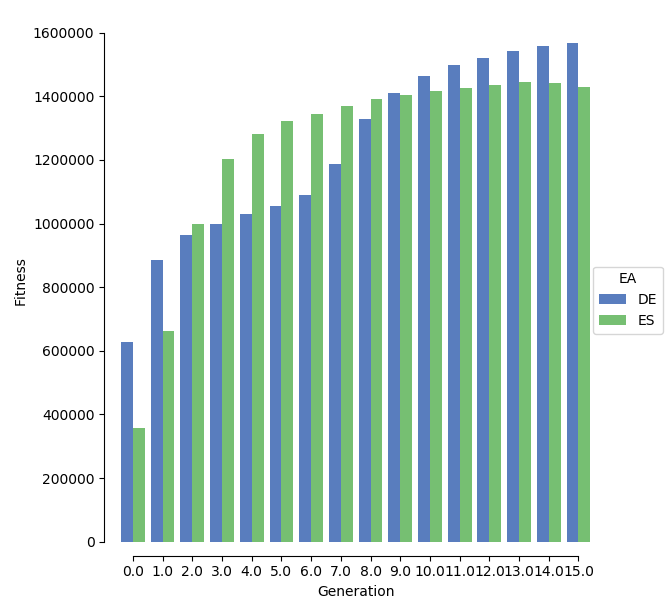
\includegraphics[width=\columnwidth]{../img/WoodMap/DEvsES/WCuttorCutMem.png}
			\caption{Scout kácení - porovnání průměrné fitness ES a DE}
			\label{obr04:CutESvsDE}
		\end{figure}
		\redo{Opravit obrázky}
		\begin{figure}[p]
			\centering
			\begin{subfigure}{.5\textwidth}
				\centering
				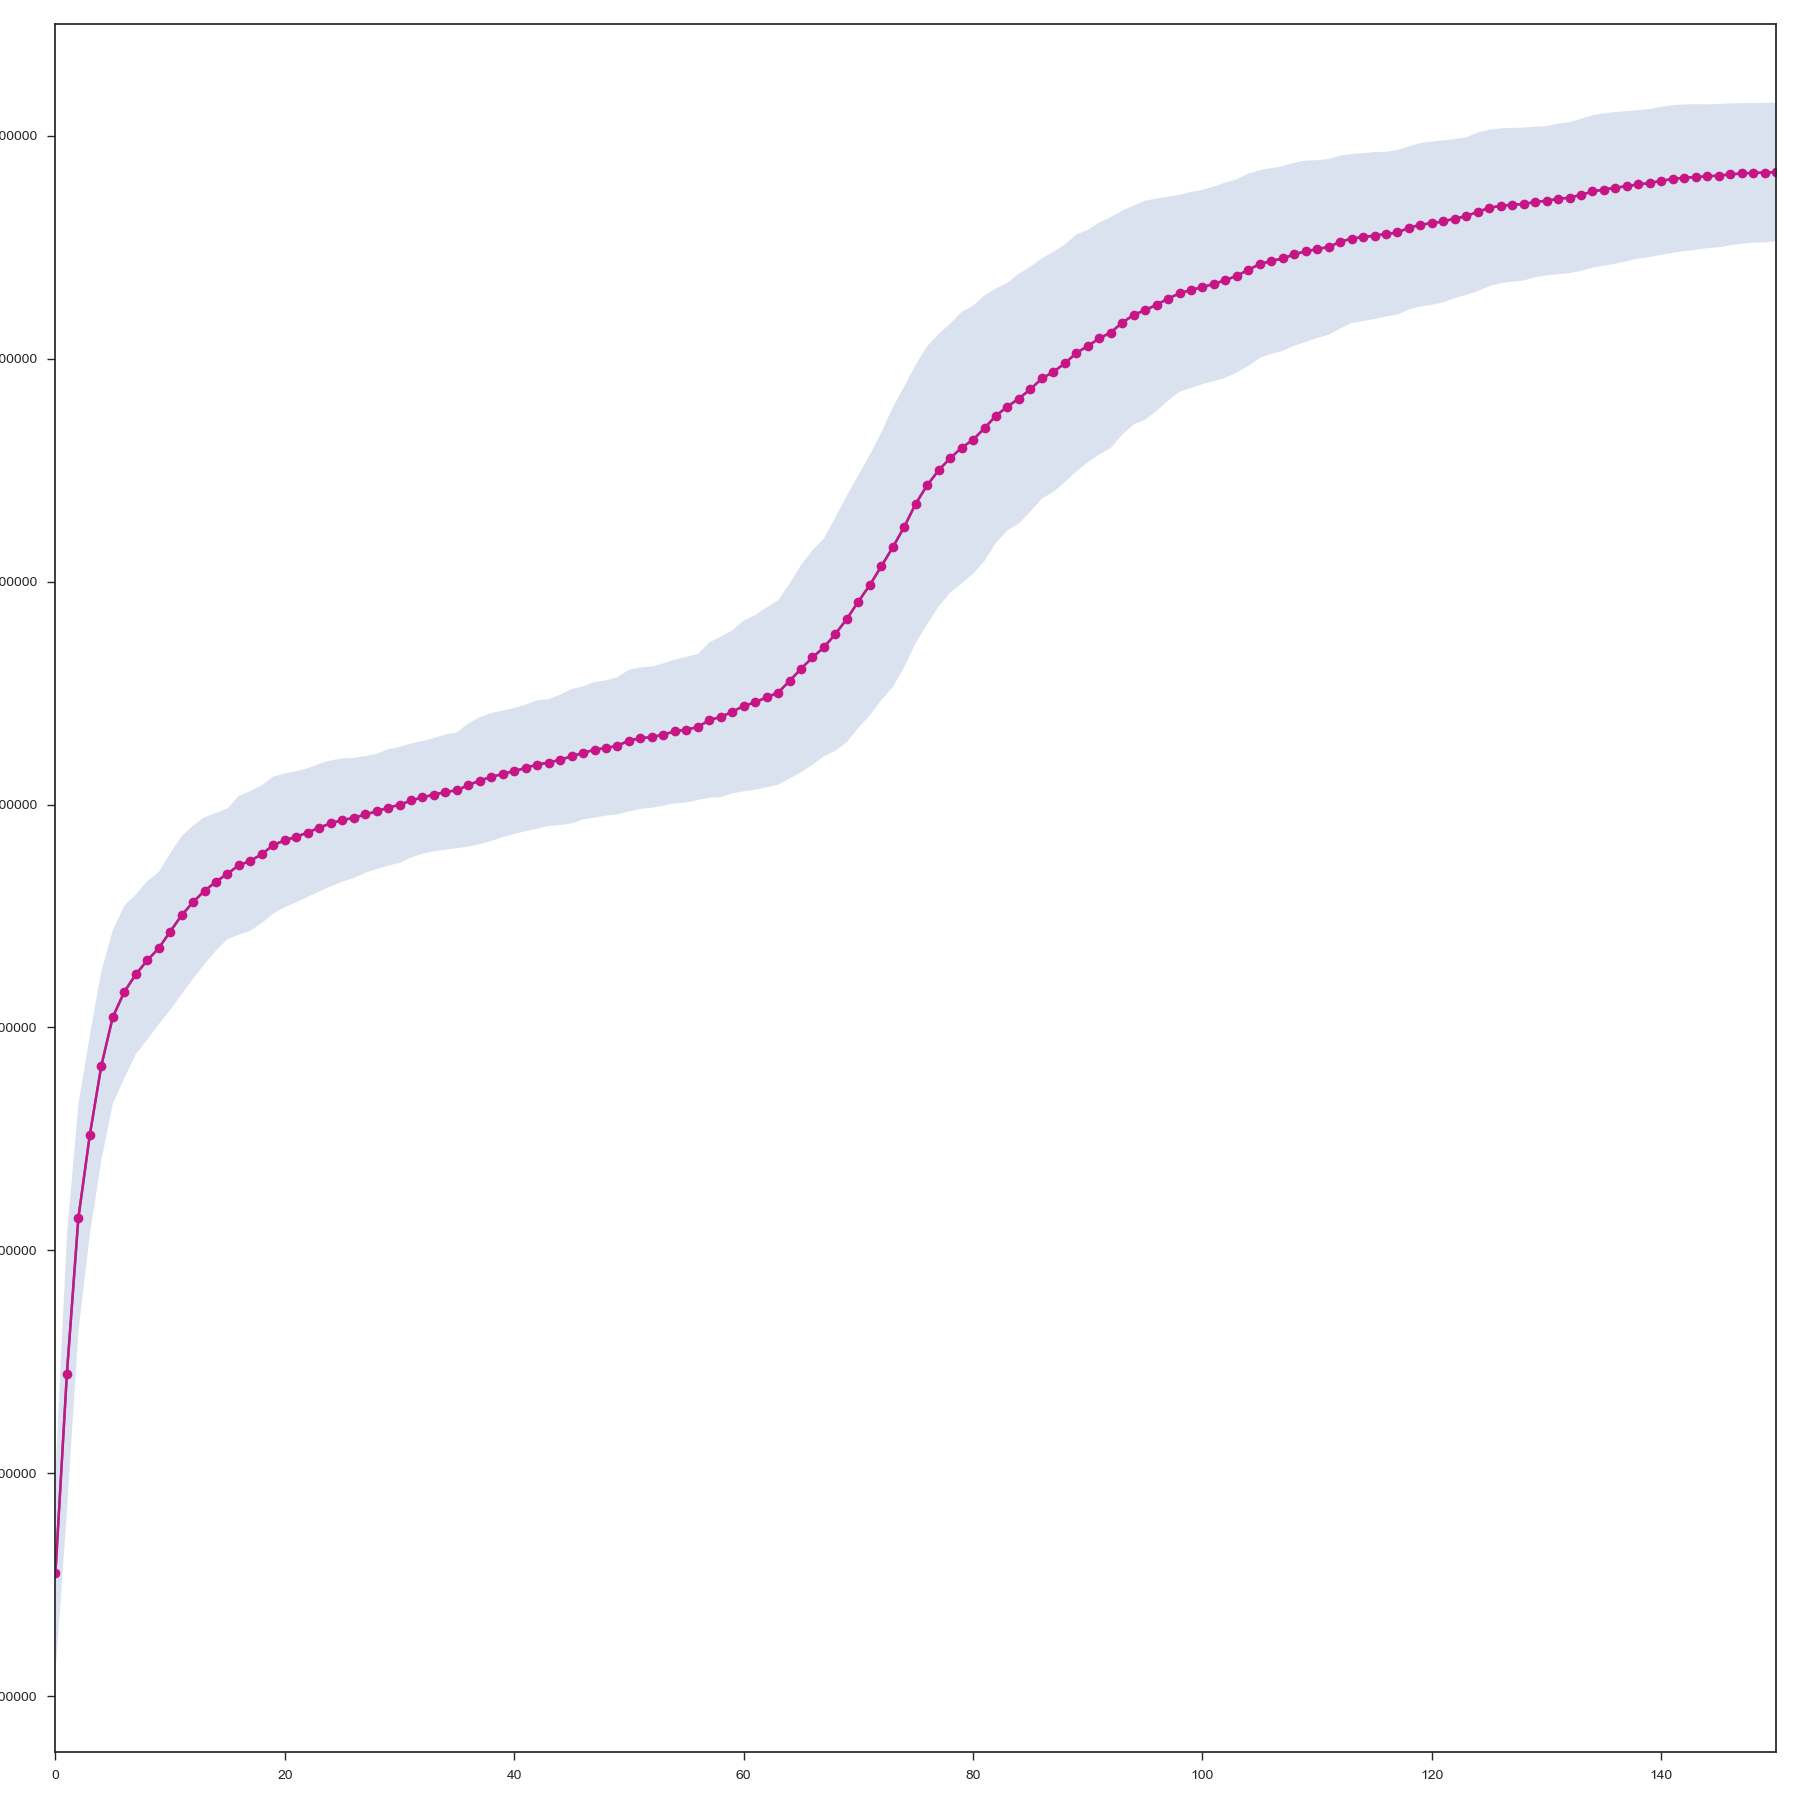
\includegraphics[width=\linewidth]{../img/WoodMap/DE/graph_of_CuttorCut-mean.png}
				\caption{DE}
				\label{obr04:CutDE}
			\end{subfigure}%
			\begin{subfigure}{.5\textwidth}
				\centering
				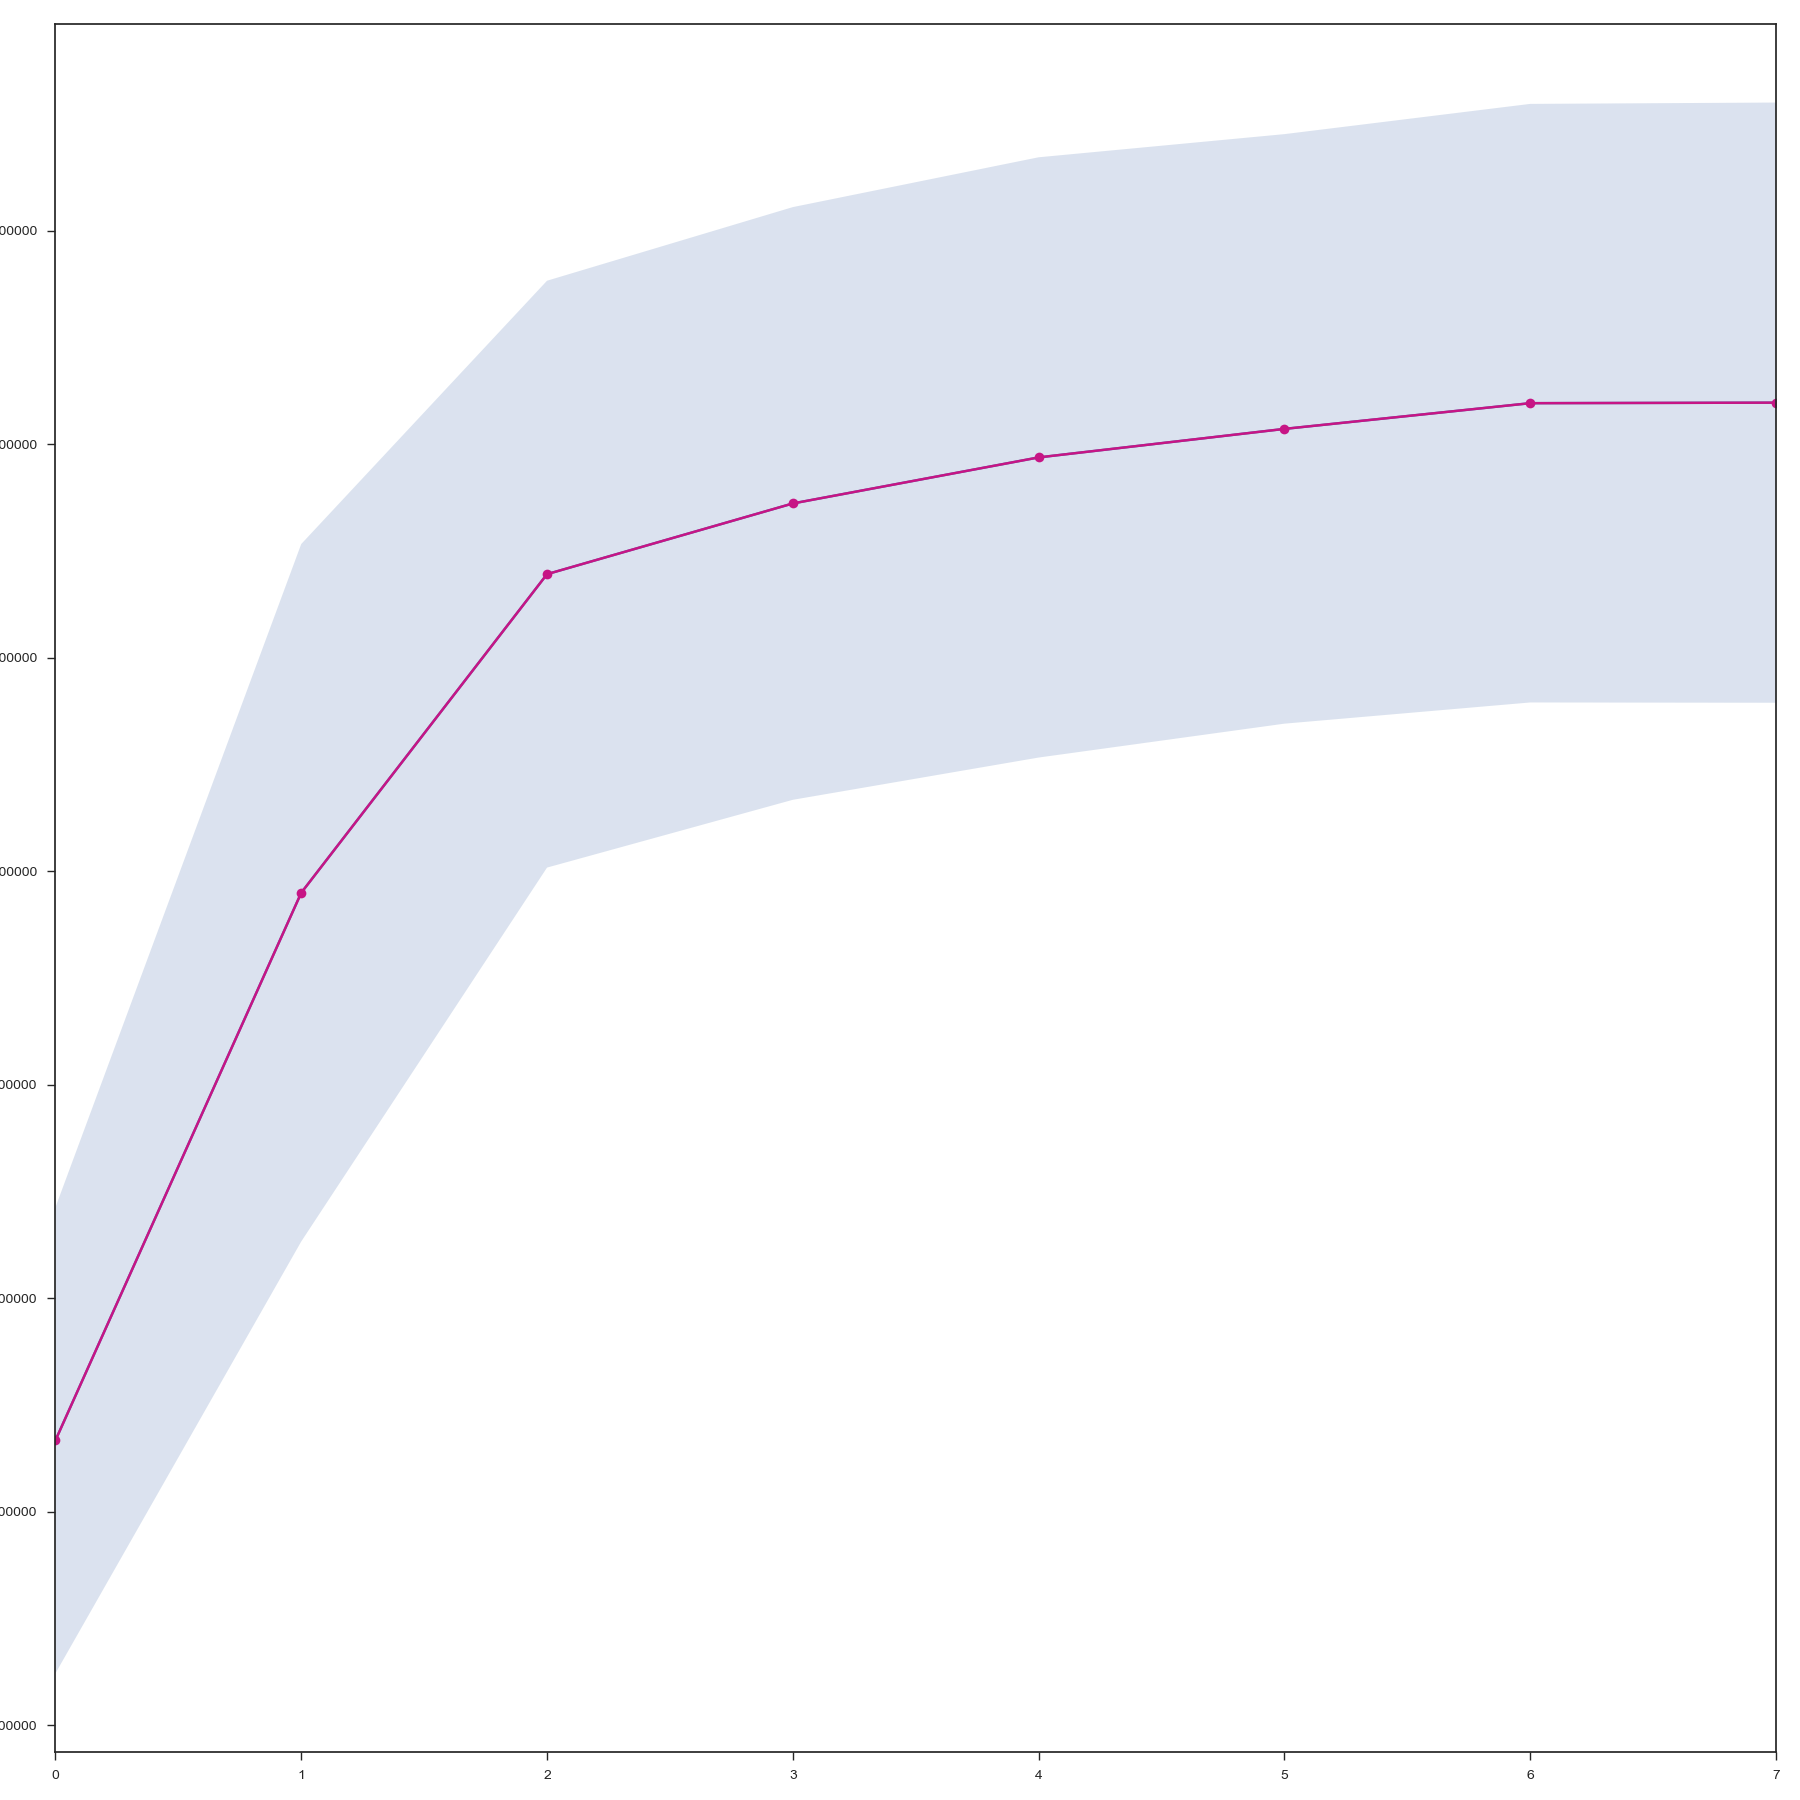
\includegraphics[width=\linewidth]{../img/WoodMap/ES/WoodCutES-mean.png}
				\caption{ES}
				\label{obr04:CutES}
			\end{subfigure}
			\caption{Scout kácení - průběh fitness v rámci generací}
			\label{obr04:Cut}
		\end{figure}
		\clearpage

	\subsubsection{Worker sbírání - nastavení experimentu}
	\begin{table}[h]\centering
	\begin{tabular}{l@{\hspace{1.5cm}}D{.}{,}{3.2}D{.}{,}{1.2}D{.}{,}{2.3}}
		\toprule
		& \mc{} & \mc{}\\
		\pulrad{\textbf{Vlastnost:}} & \mc{\pulrad{\textbf{Hodnota:}}}\\
		\midrule
		Roboti:     & Worker-4 \\
		Počet generací: & 2000\\
		Počet iterací map & 1000\\
		Velikost generace(DE) & 200\\
		Počet jedinců(ES) & 10\\
		Počet mutovaný potomků(ES)&20\\
		Elitismus(ES)& Ano\\
		Elitismus(DE)& Ne \\
		\bottomrule
		\multicolumn{2}{l}{\footnotesize \textit{Pozn:}
			Nastavení evolučních algoritmů}
	\end{tabular}
	\par 
	\begin{tabular}{l@{\hspace{1.5cm}}D{.}{,}{3.2}D{.}{,}{1.2}D{.}{,}{2.3}}
		\toprule
		& \mc{} & \mc{}\\
		\pulrad{\textbf{Vlastnost:}} & \mc{\pulrad{\textbf{Hodnota:}}}\\
		\midrule
		Hodnota nalezeného pokáceného stromu &  100 \\
		Hodnota uloženého dřeva & 1010\\
		Hodnota dřeva v kontejneru & 1000\\
		Hodnota jiné entity v kontejneru & -100\\
		Hodnota kolize & -1\\
		Ostatní hodnoty: & 0\\
		Počet stromů: & 200\\
		Počet už pokácených stromů & 200\\
		\bottomrule
		\multicolumn{2}{l}{\footnotesize \textit{Pozn:}
			Nastavení hodnocení fitness}
	\end{tabular}
	\caption{Worker sbírání - nastavení experimentu}
	\end{table}
	\begin{figure}[t]\centering       
		\includegraphics[width=\columnwidth]{../img/WoodMap/DEvsES/PickUp.png}
		\caption{ Worker sbírání - porovnání průměrné fitness ES a DE}
		\label{obr04:PickupESvsDE}
	\end{figure}
	\redo{Opravit obrázky
	}\begin{figure}[p]
		\centering
		\begin{subfigure}{.5\textwidth}
			\centering
			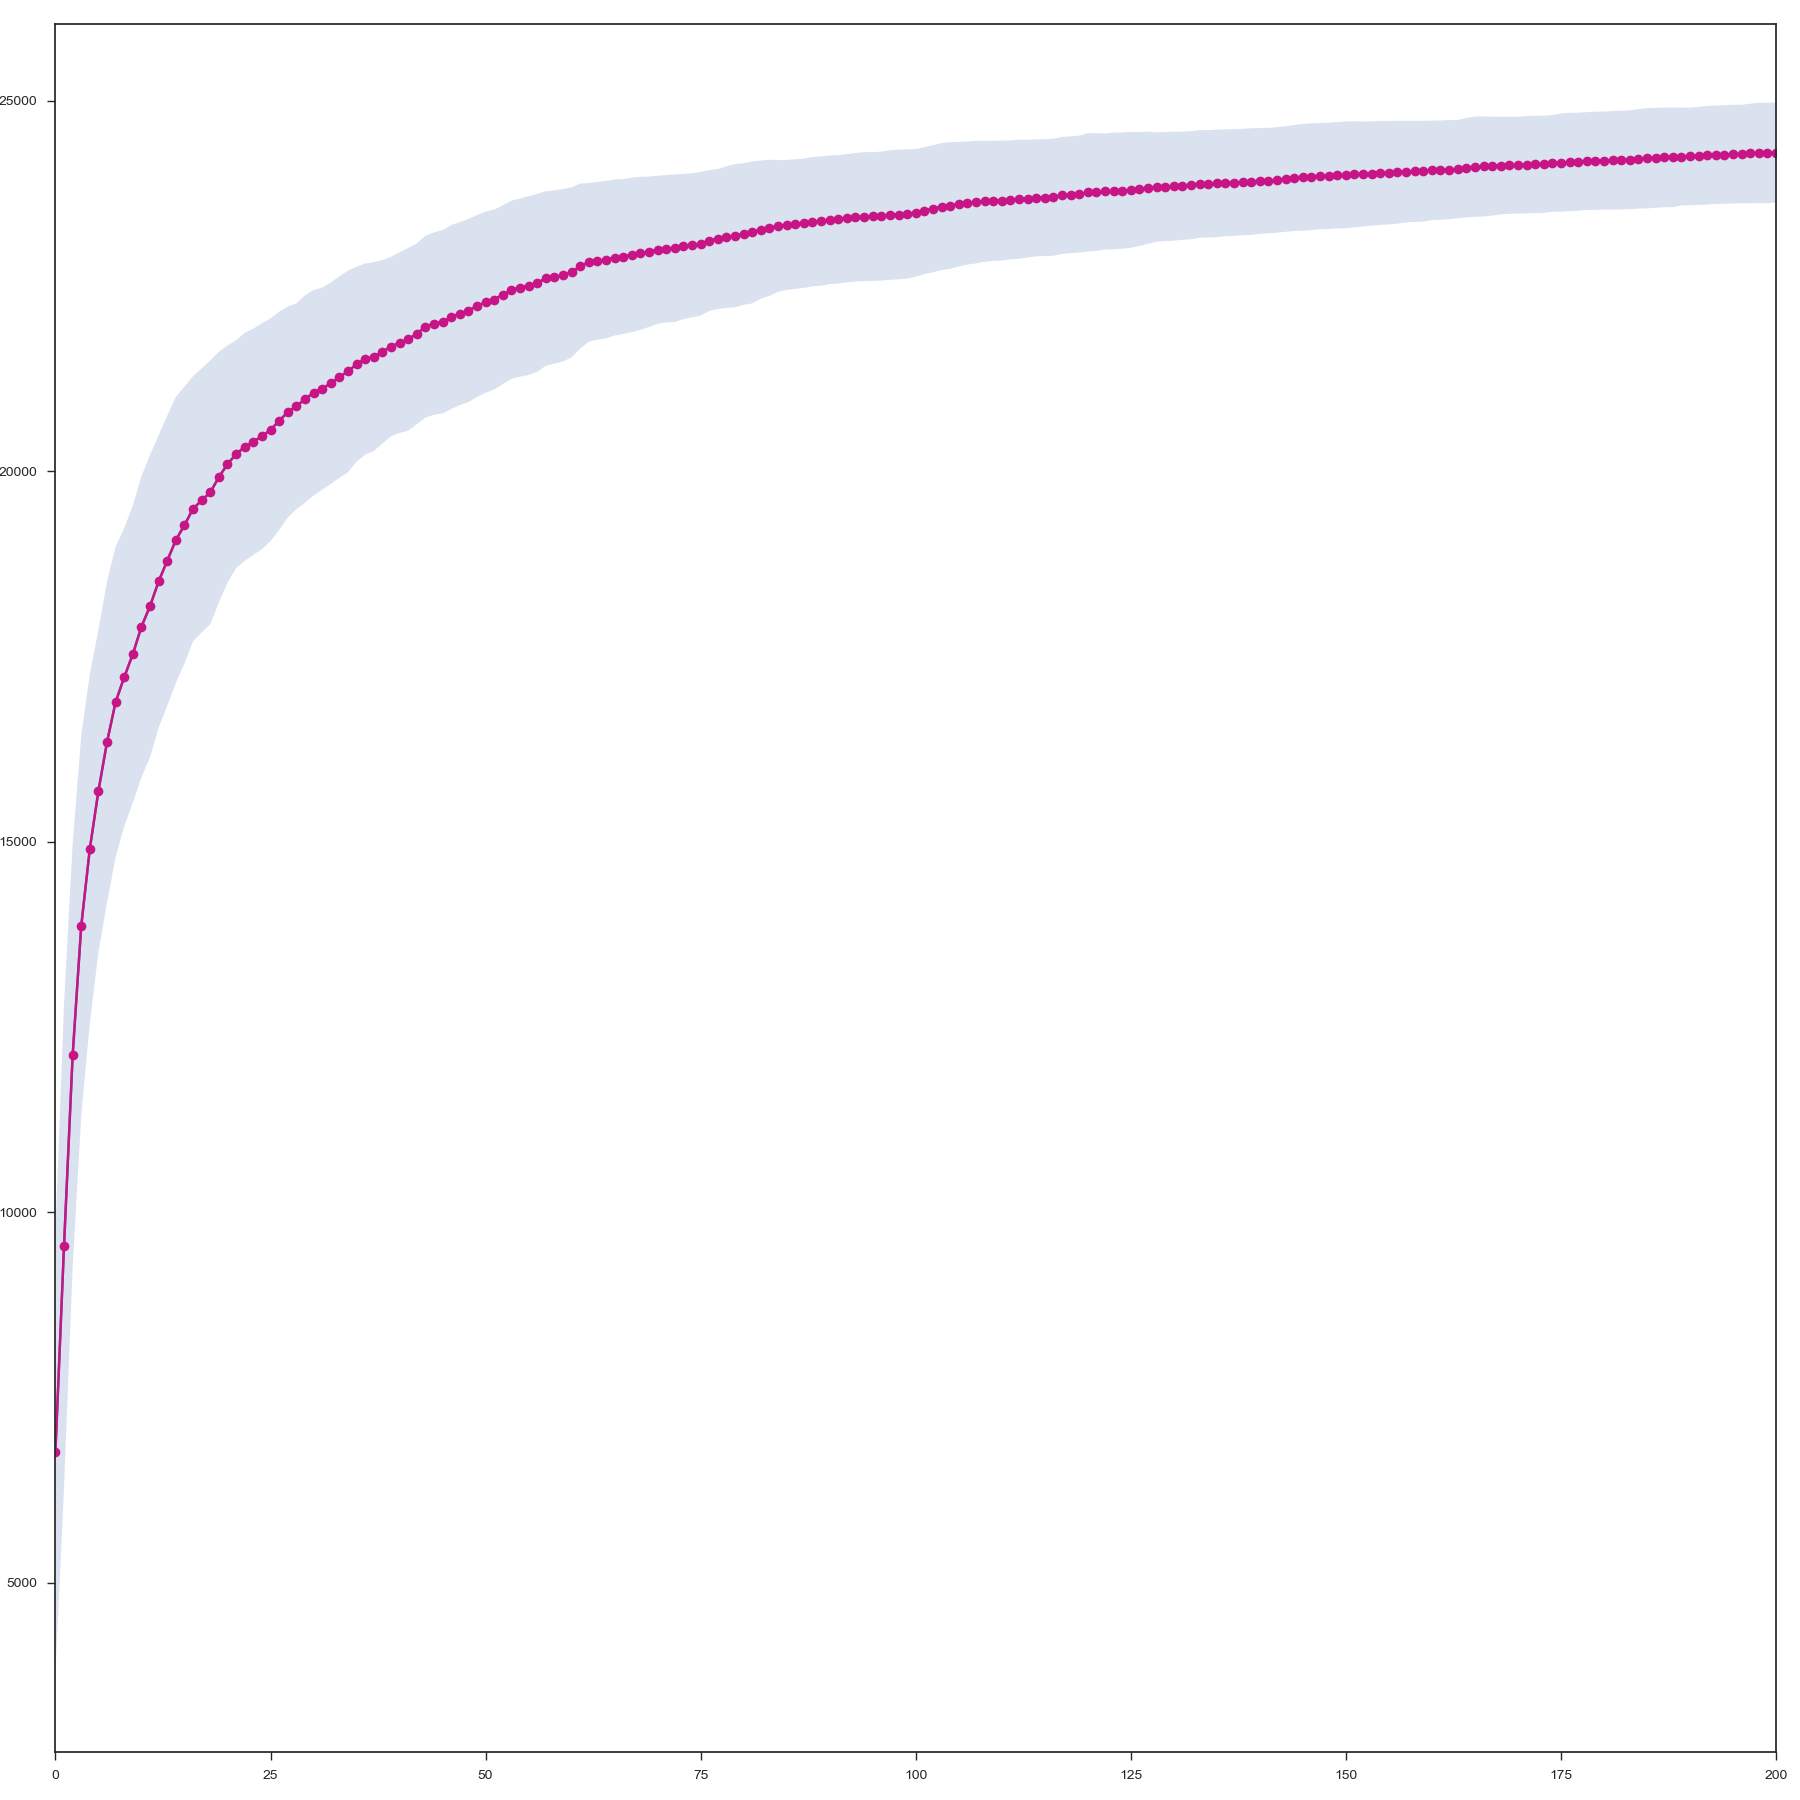
\includegraphics[width=\linewidth]{../img/WoodMap/DE/graph_of_WorkerPickUpMem-mean.png}
			\caption{DE}
			\label{obr04:PickupDE}
		\end{subfigure}%
		\begin{subfigure}{.5\textwidth}
			\centering
			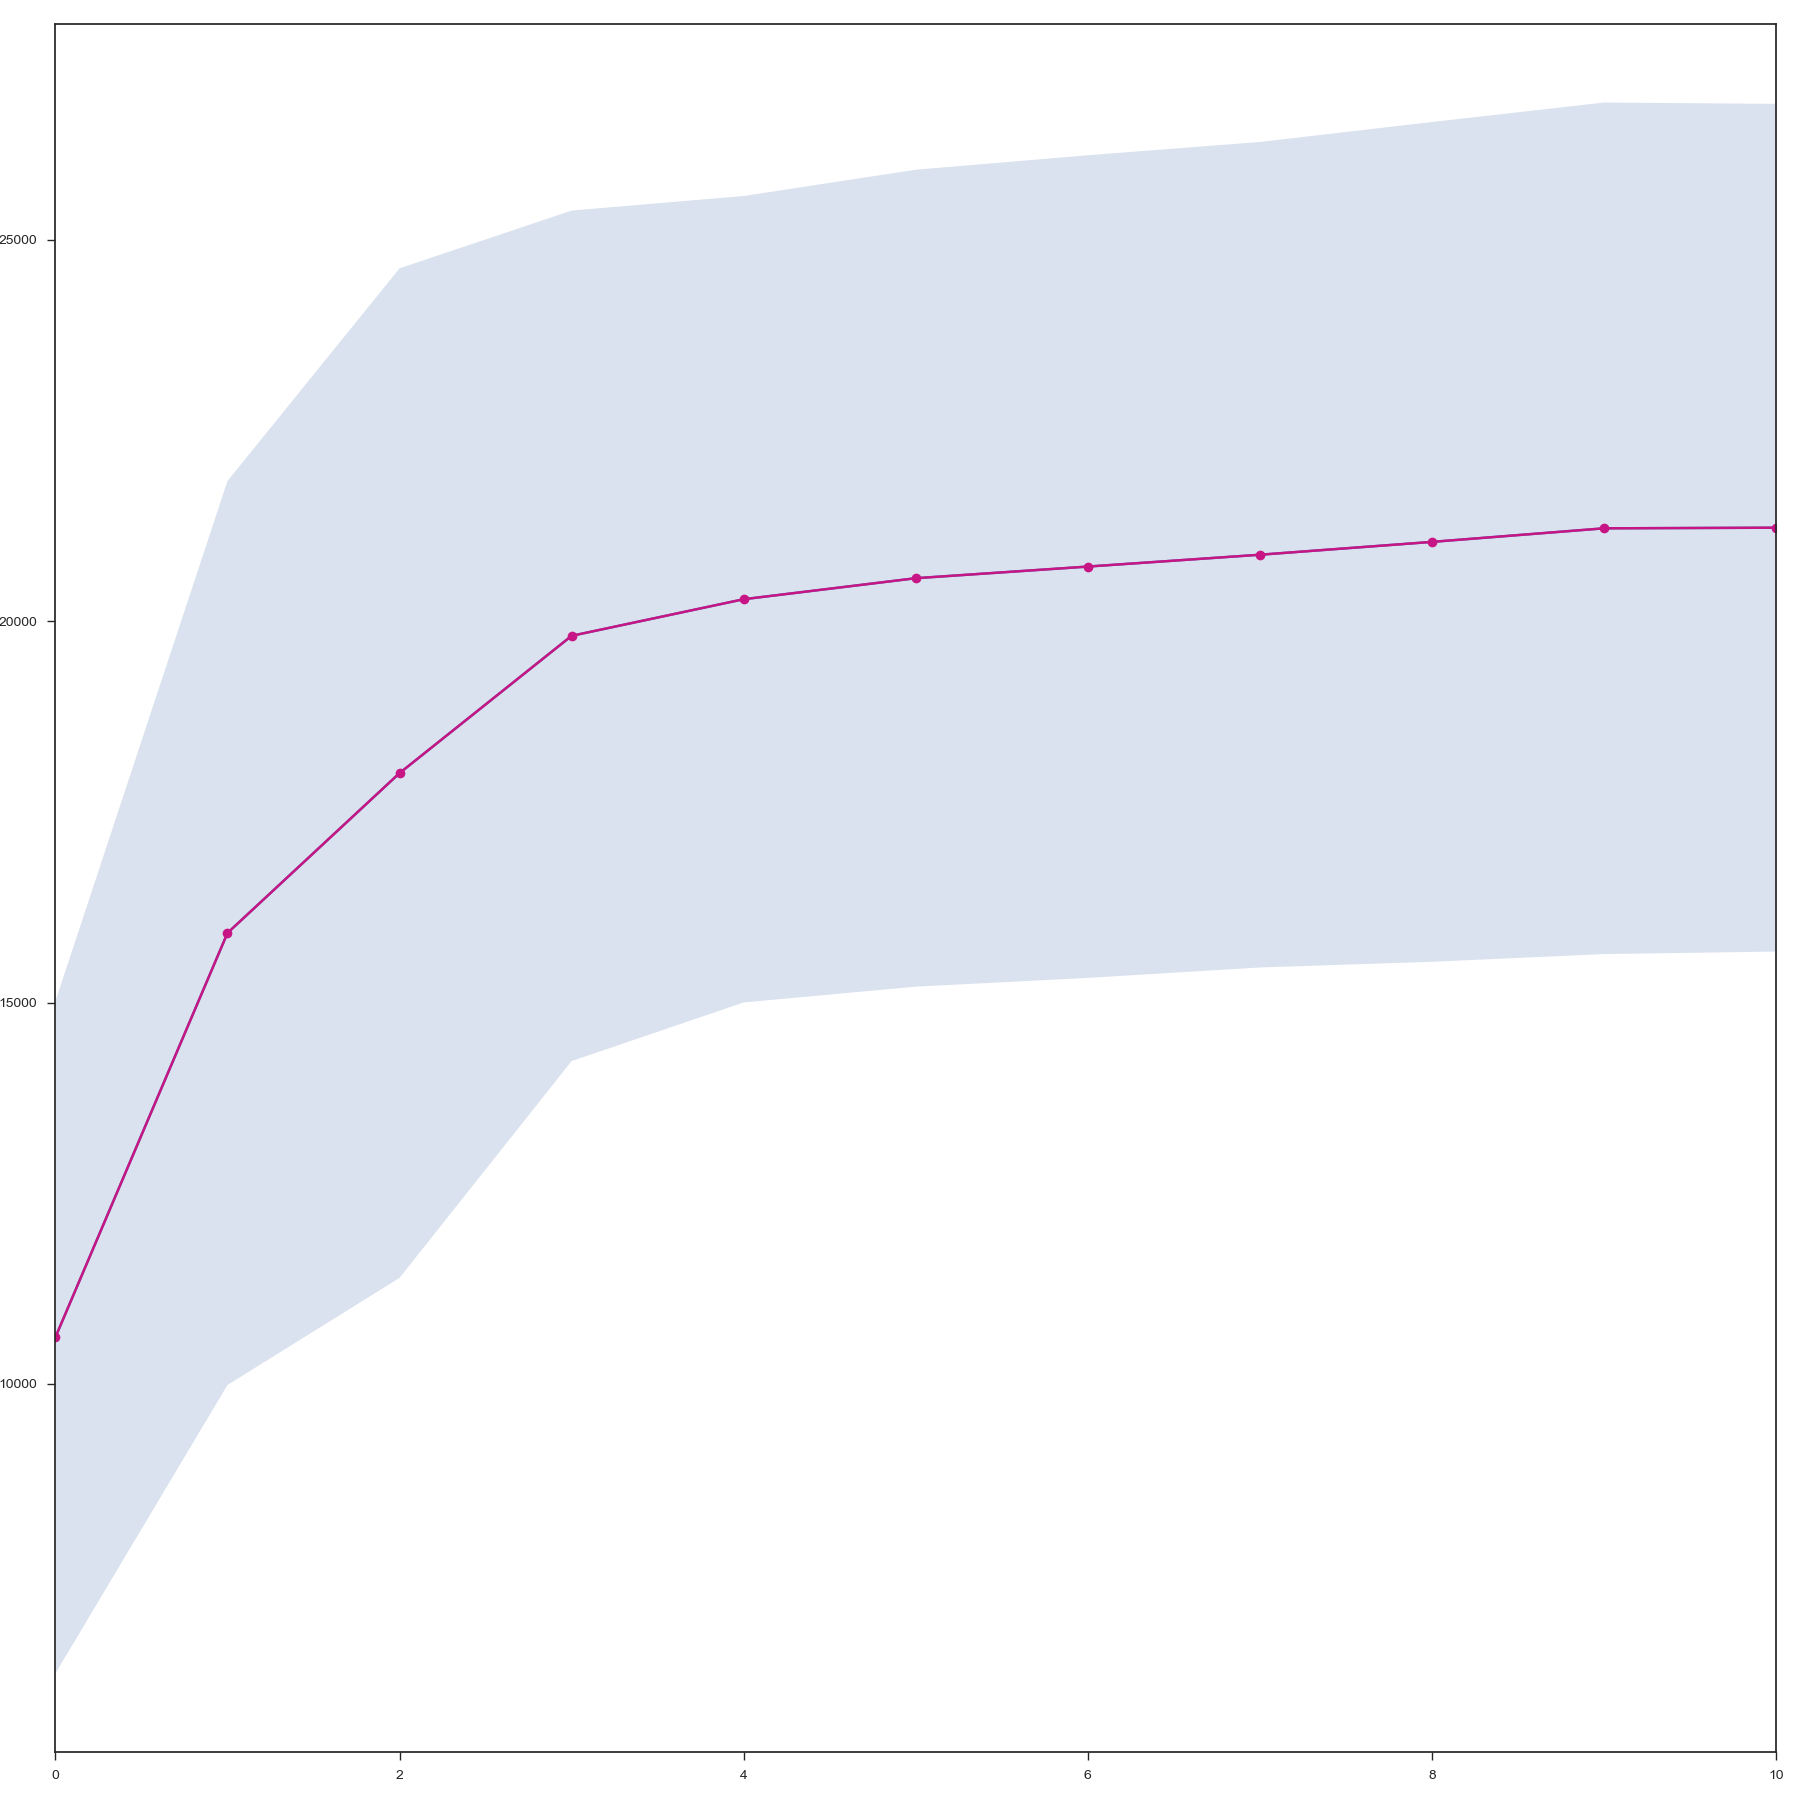
\includegraphics[width=\linewidth]{../img/WoodMap/ES/WoodPickupES-mean.png}
			\caption{ES}
			\label{obr04:PickupES}
		\end{subfigure}
		\caption{Worker sbírání - průběh fitness v rámci generací}
		\label{obr04:Pickup}
	\end{figure}
	\clearpage
	\subsubsection{Worker ukládání doprostřed  - nastavení experimentu}
	\begin{table}[h]\centering   
		\begin{tabular}{l@{\hspace{1.5cm}}D{.}{,}{3.2}D{.}{,}{1.2}D{.}{,}{2.3}}
			\toprule
			& \mc{} & \mc{}\\
			\pulrad{\textbf{Vlastnost:}} & \mc{\pulrad{\textbf{Hodnota:}}}\\
			\midrule
			Roboti:     & Worker-4 \\
			Počet generací: & 2000\\
			Počet iterací map & 2000\\
			Velikost generace(DE) & 200\\
			Počet jedinců(ES) & 10\\
			Počet mutovaný potomků(ES)&20\\
			Elitismus(ES)& Ano\\
			Elitismus(DE)& Ne \\
			\bottomrule
			\multicolumn{2}{l}{\footnotesize \textit{Pozn:}
				Nastavení evolučních algoritmů}
		\end{tabular}
		\par 
		\begin{tabular}{l@{\hspace{1.5cm}}D{.}{,}{3.2}D{.}{,}{1.2}D{.}{,}{2.3}}
			\toprule
			& \mc{} & \mc{}\\
			\pulrad{\textbf{Vlastnost:}} & \mc{\pulrad{\textbf{Hodnota:}}}\\
			\midrule
			Hodnota nalezeného pokáceného stromu &  100 \\
			Hodnota uloženého dřeva & 1000\\
			Hodnota dřeva v kontejneru & 100\\
			Hodnota jiné entity v kontejneru & -100\\
			Hodnota kolize & -1\\
			Ostatní hodnoty: & 0\\
			Počet stromů: & 200\\
			Počet už pokácených stromů & 200\\
			\bottomrule
			\multicolumn{2}{l}{\footnotesize \textit{Pozn:}
				Nastavení hodnocení fitness}
		\end{tabular}
		\caption{Worker ukládání doprostřed  - nastavení experimentu}
	\end{table}
	\begin{figure}[t]\centering
		\includegraphics[width=\columnwidth]{../img/WoodMap/DEvsES/Stock.png}
		\caption{Worker ukládání doprostřed  - porovnání průměrné fitness ES a DE}
		\label{obr04:StockESvsDE}
	\end{figure}
	\redo{Opravit obrázky
	}\begin{figure}[p]
		\centering
		\begin{subfigure}{.5\textwidth}
			\centering
			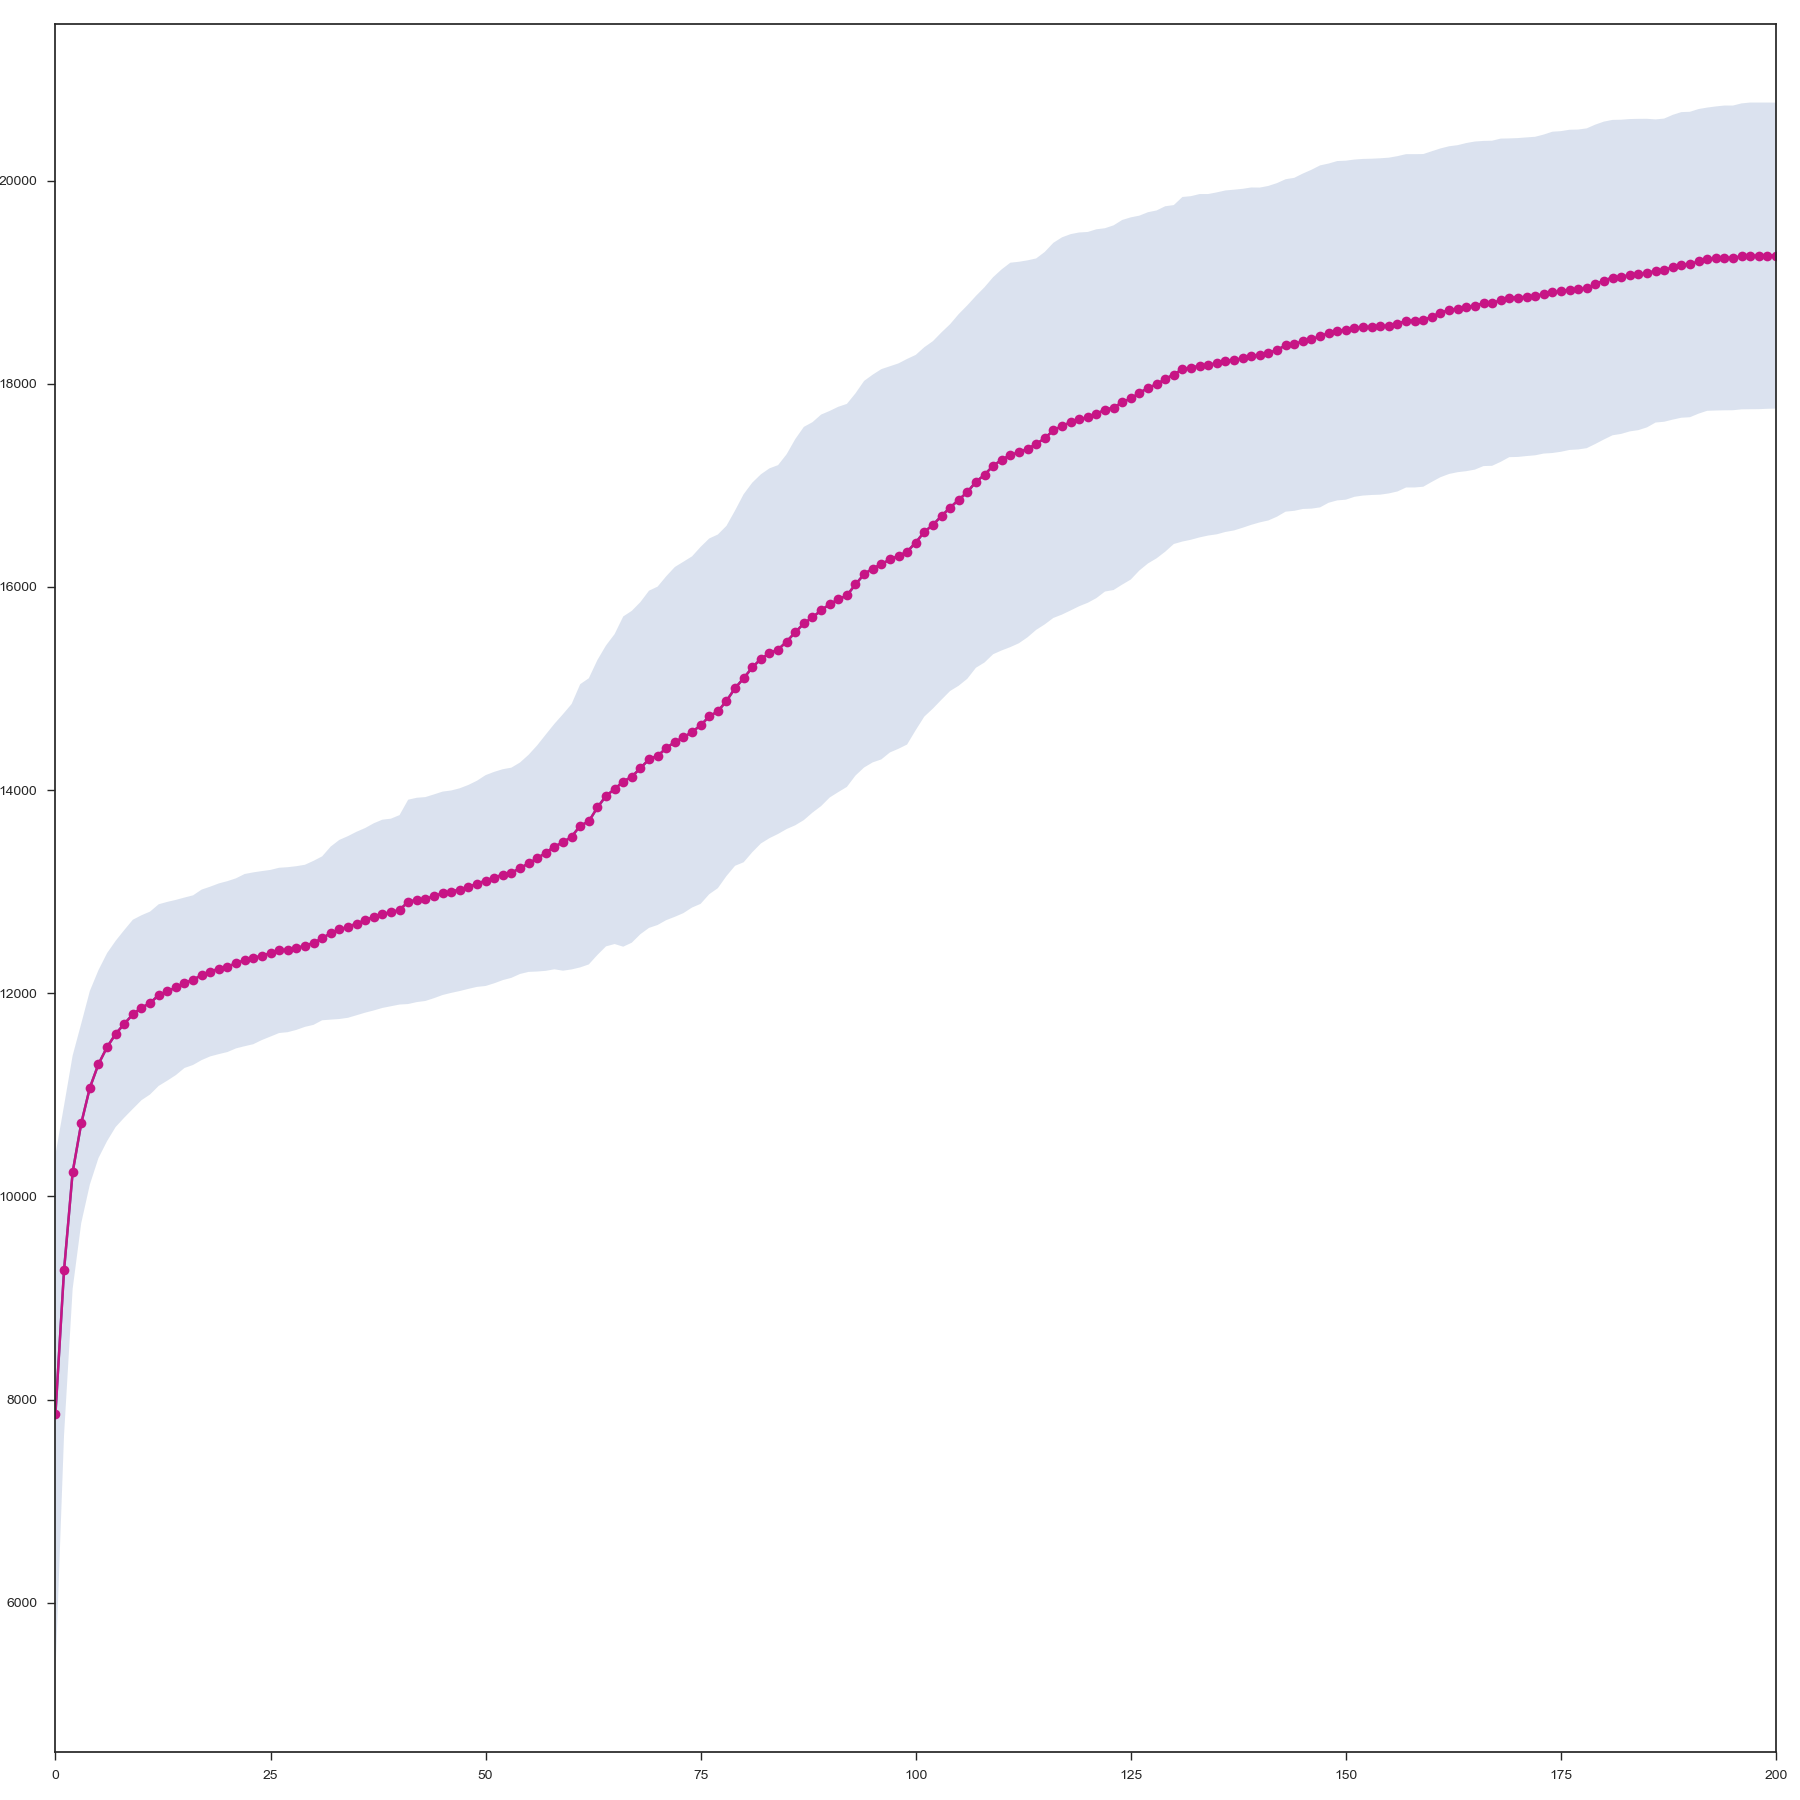
\includegraphics[width=\linewidth]{../img/WoodMap/DE/graph_of_WorkerStockMem-mean.png}
			\caption{DE}
			\label{obr04:StockDE}
		\end{subfigure}%
		\begin{subfigure}{.5\textwidth}
			\centering
			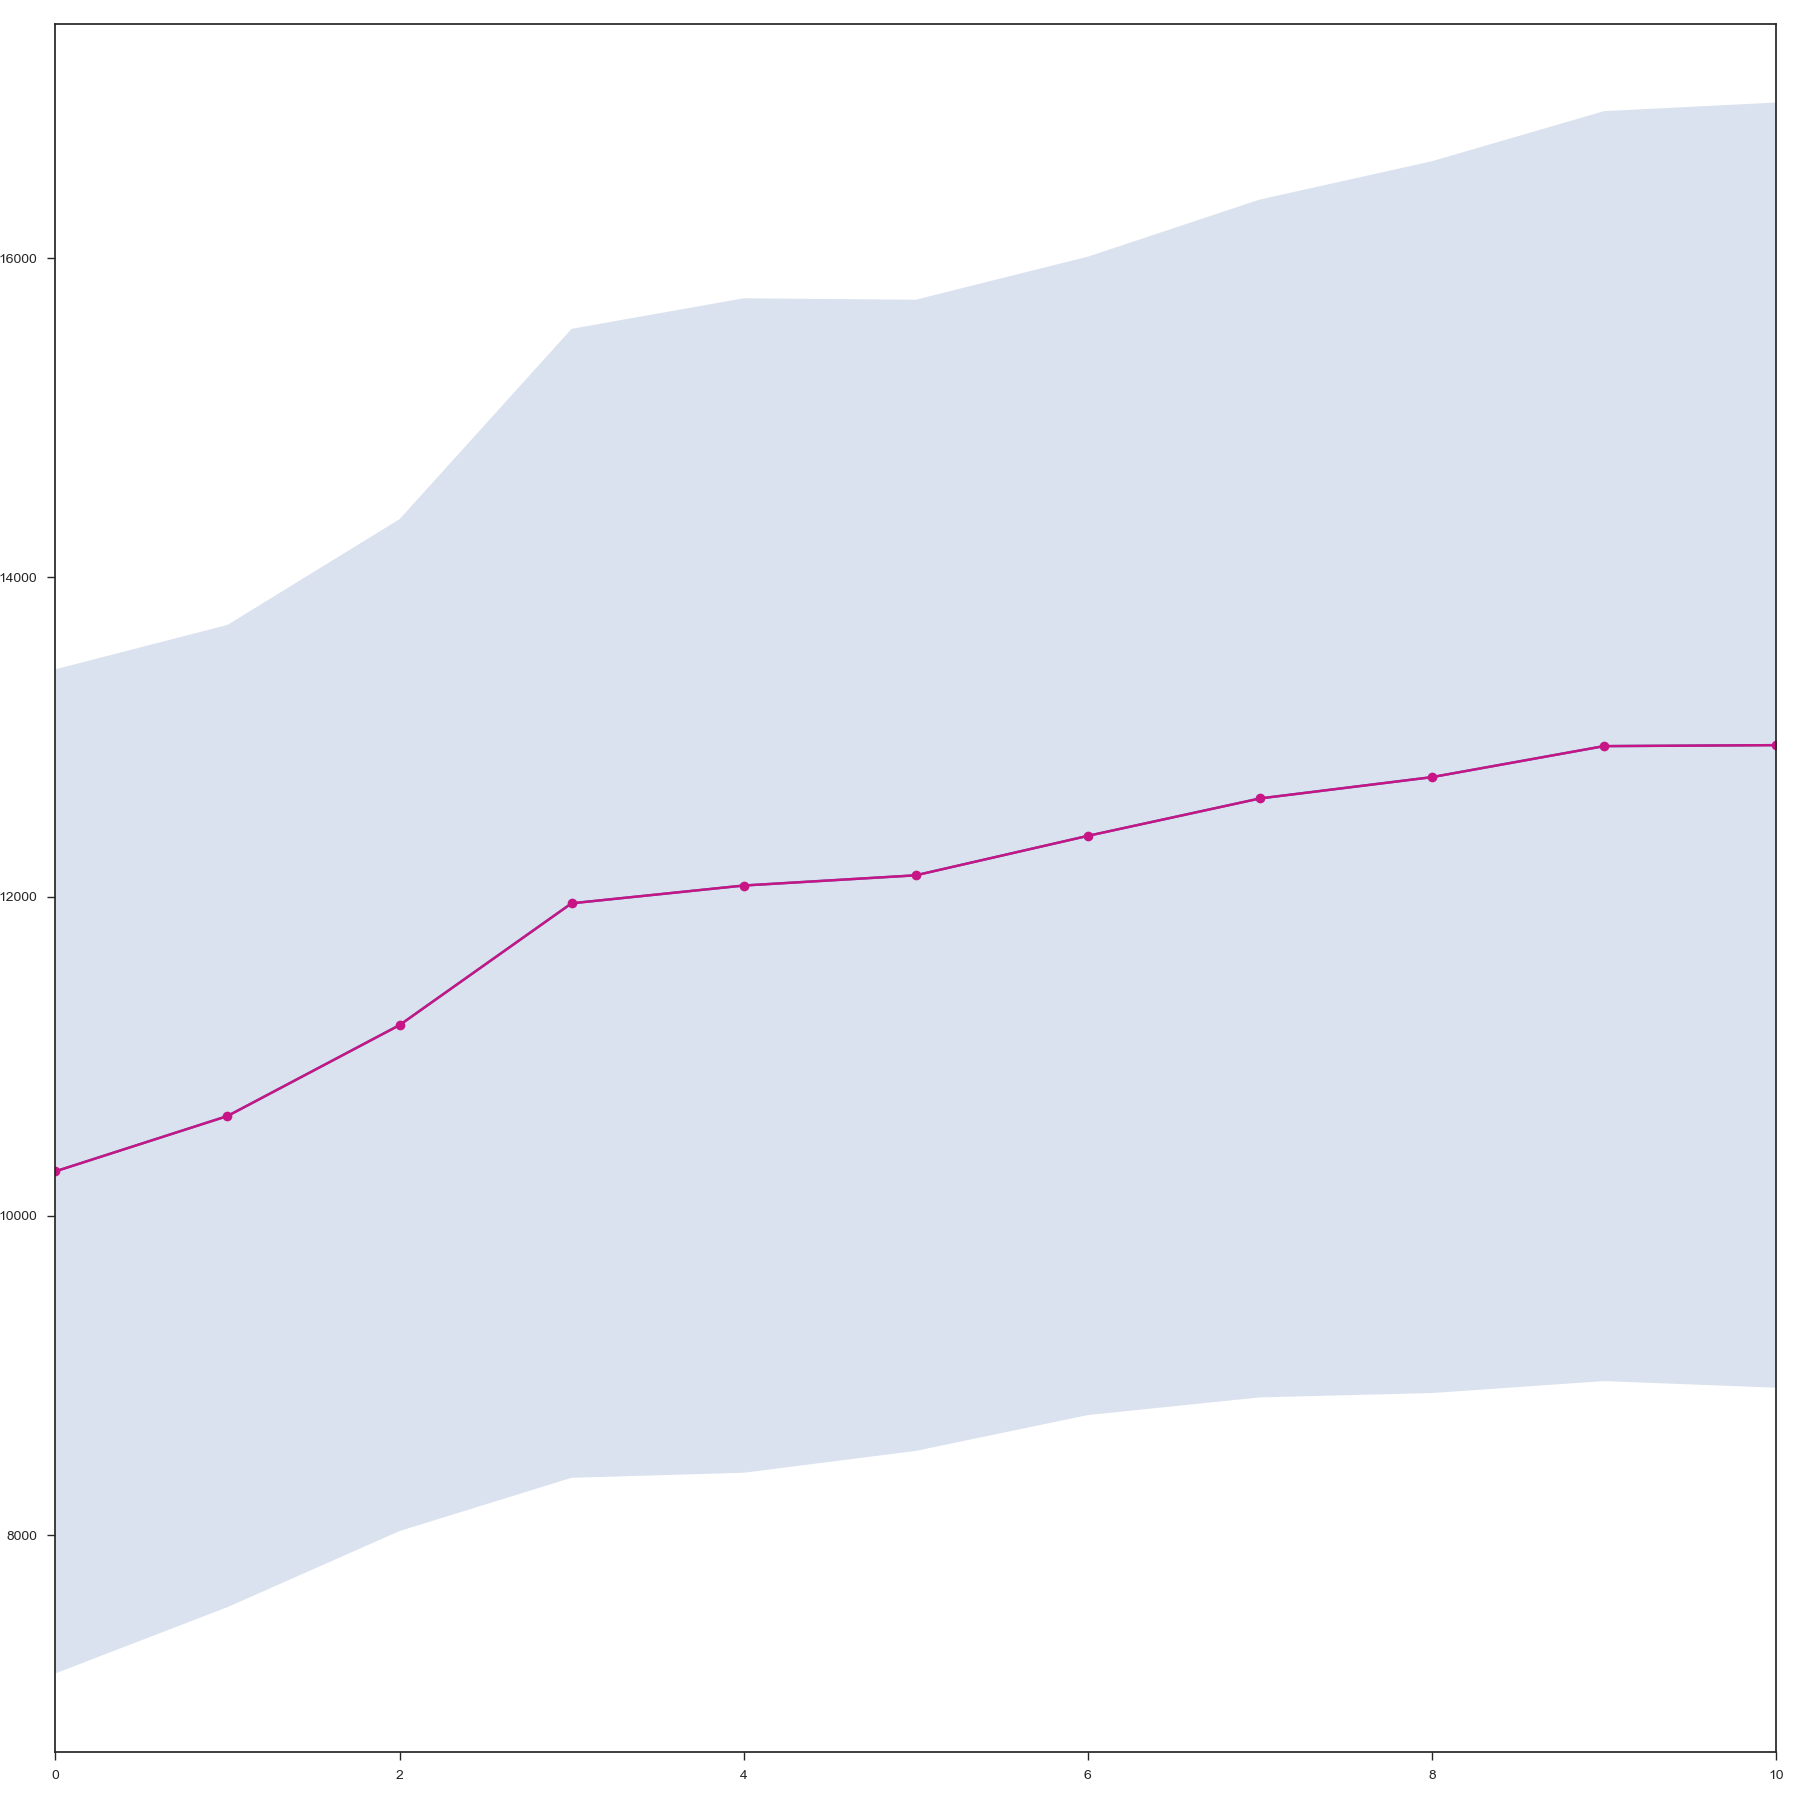
\includegraphics[width=\linewidth]{../img/WoodMap/ES/WoodStockES-mean.png}
			\caption{ES}
			\label{obr04:StockES}
		\end{subfigure}
		\caption{Worker ukládání doprostřed  - Průběh fitness v rámci generací}
		\label{obr04:Stock}
	\end{figure}
	\clearpage
	\subsubsection{Kooperace  hlavní úkol  - nastavení experimentu}
	\begin{table}[h]\centering
		\begin{tabular}{l@{\hspace{1.5cm}}D{.}{,}{3.2}D{.}{,}{1.2}D{.}{,}{2.3}}
			\toprule
			& \mc{} & \mc{}\\
			\pulrad{\textbf{Vlastnost:}} & \mc{\pulrad{\textbf{Hodnota:}}}\\
			\midrule
			Roboti:     & Scout-5, Worker-4 \\
			Počet generací: & 4000\\
			Počet iterací map & 2000\\
			Velikost generace(DE) & 200\\
			Počet jedinců(ES) & 10\\
			Počet mutovaný potomků(ES)&20\\
			Elitismus(ES)& Ano\\
			Elitismus(DE)& Ne \\
			\bottomrule
			\multicolumn{2}{l}{\footnotesize \textit{Pozn:}
				Nastavení evolučních algoritmů}
		\end{tabular}
		\par 
		\begin{tabular}{l@{\hspace{1.5cm}}D{.}{,}{3.2}D{.}{,}{1.2}D{.}{,}{2.3}}
			\toprule
			& \mc{} & \mc{}\\
			\pulrad{\textbf{Vlastnost:}} & \mc{\pulrad{\textbf{Hodnota:}}}\\
			\midrule
			Hodnota nalezeného pokáceného stromu &  100 \\
			Hodnota uloženého dřeva & 1000\\
			Hodnota dřeva v kontejneru & 100\\
			Hodnota jiné entity v kontejneru & -100\\
			Hodnota kolize & -1\\
			Ostatní hodnoty: & 0\\
			Počet stromů: & 400\\
			Počet už pokácených stromů & 0\\
			\bottomrule
			\multicolumn{2}{l}{\footnotesize \textit{Pozn:}
				Nastavení hodnocení fitness}
			\caption{Kooperace  hlavní úkol  - nastavení experimentu}
		\end{tabular}
	\end{table}
	\begin{figure}[t]\centering
		\includegraphics[width=\columnwidth]{../img/WoodMap/DEvsES/WoodCoop.png}
		\caption{Kooperace  hlavní úkol  - porovnání průměrné fitness ES a DE}
		\label{obr04:CoopESvsDE}
	\end{figure}
	\redo{Opravit obrázky
	}\begin{figure}[p]
		\centering
		\begin{subfigure}{.5\textwidth}
			\centering
			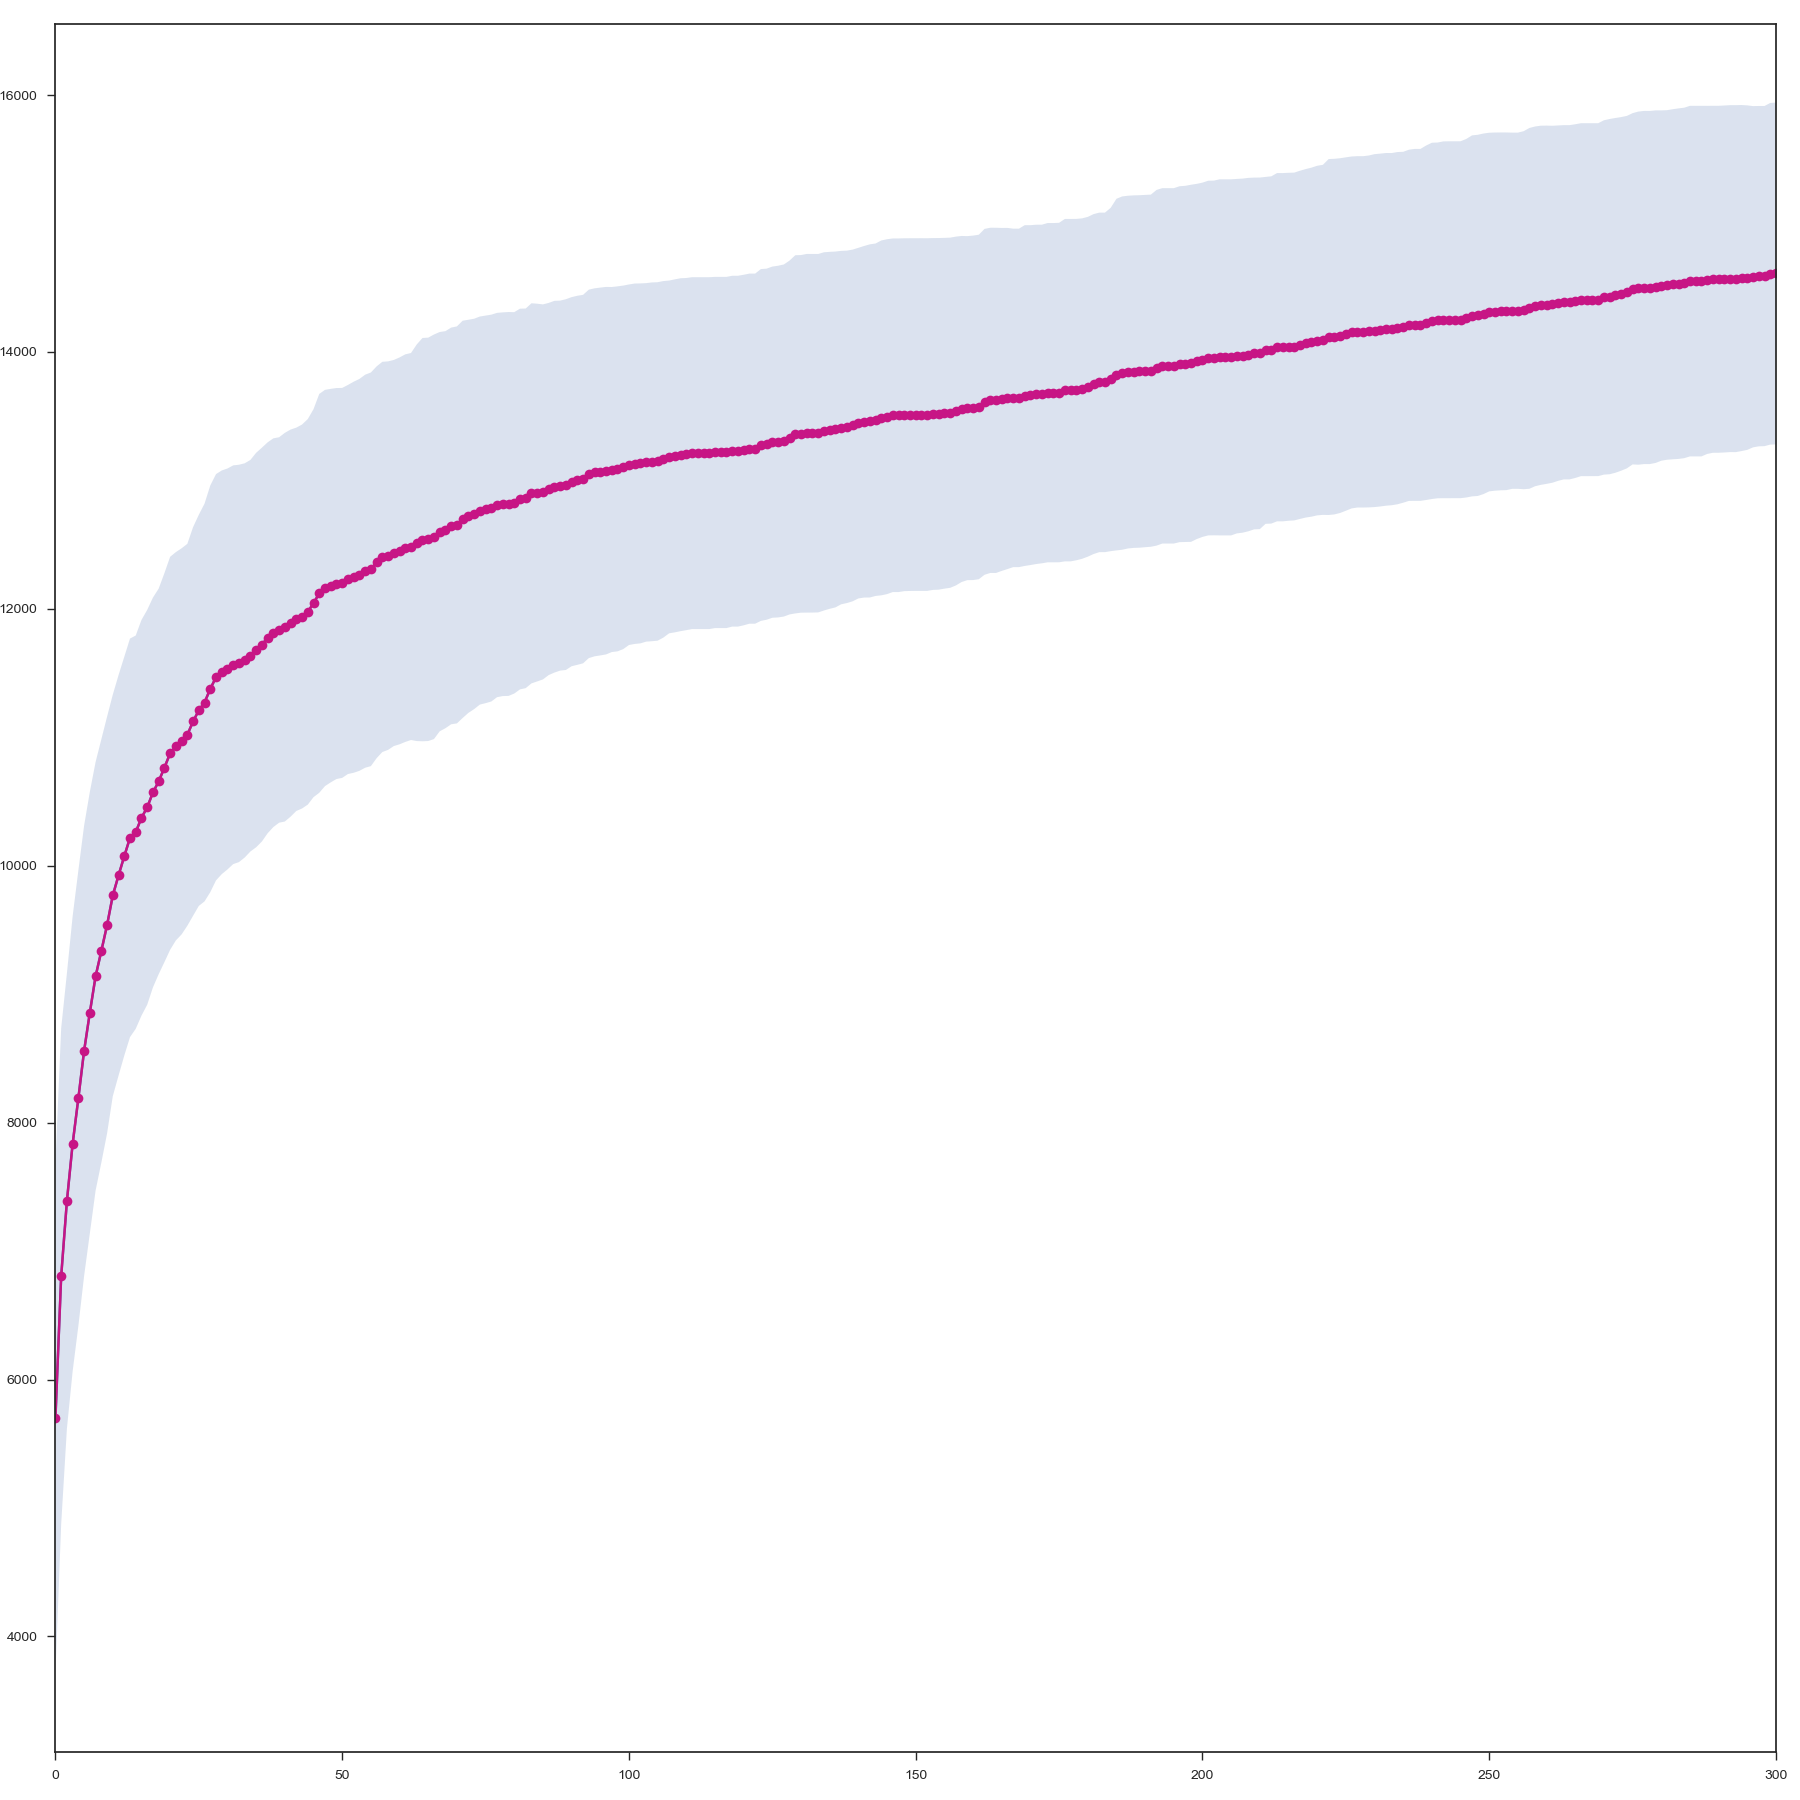
\includegraphics[width=\linewidth]{../img/WoodMap/DE/graph_of_WoodCoopMem-mean.png}
			\caption{DE}
			\label{obr04:CoopDE}
		\end{subfigure}%
		\begin{subfigure}{.5\textwidth}
			\centering
			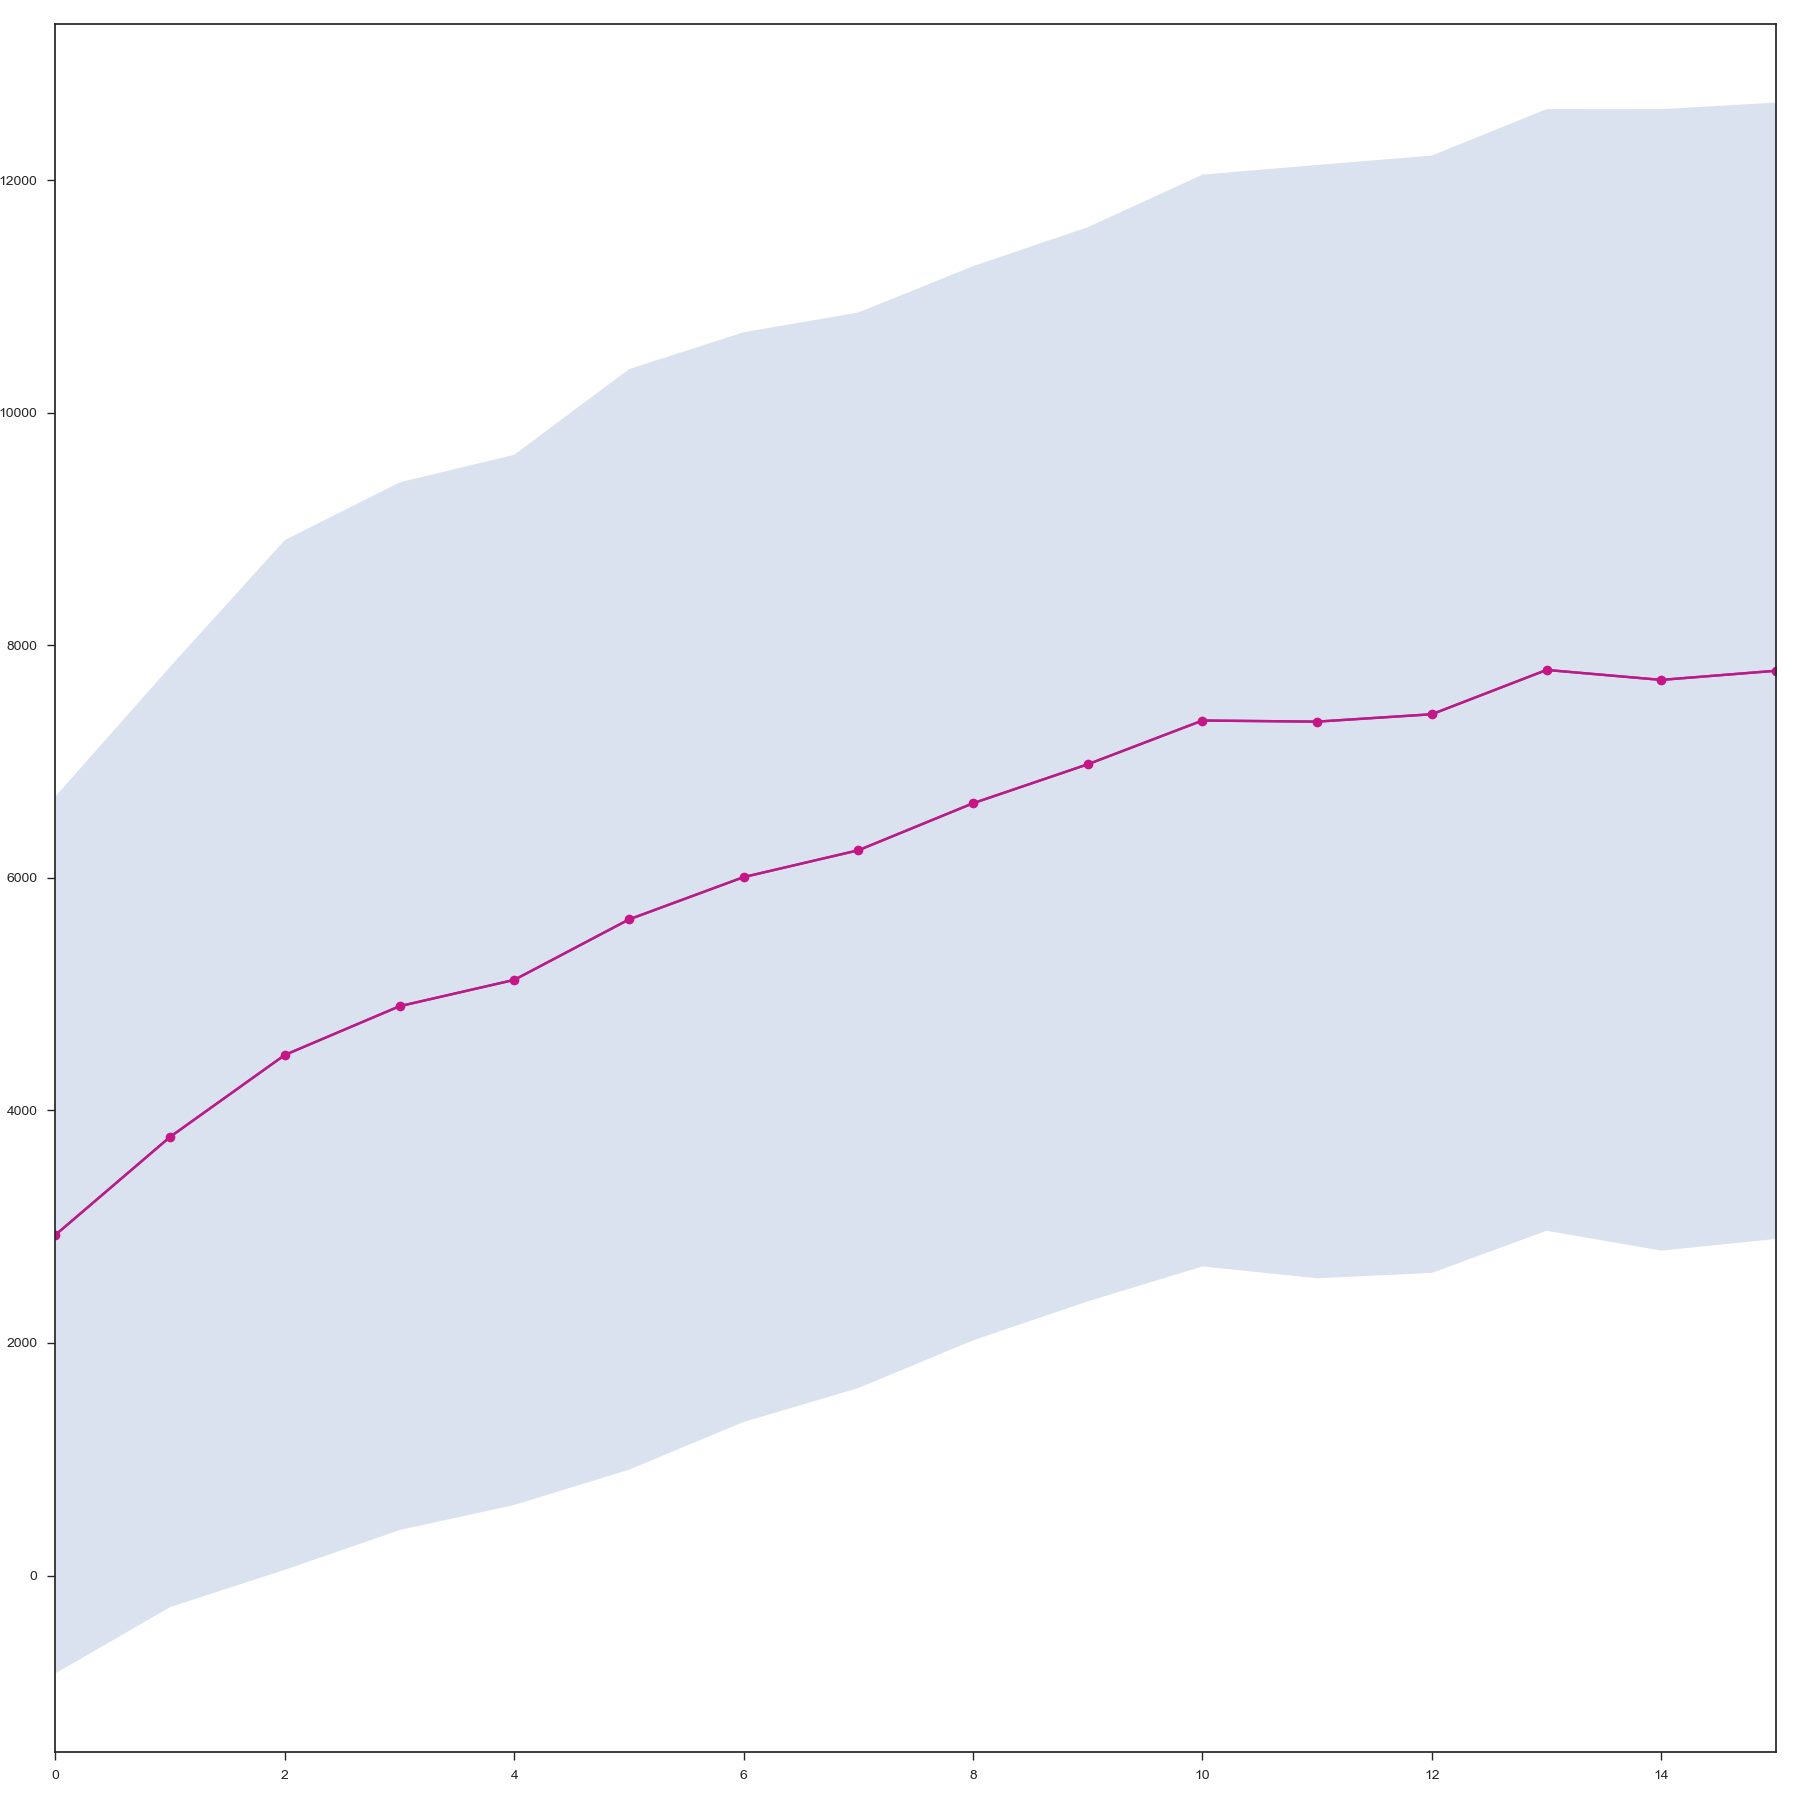
\includegraphics[width=\linewidth]{../img/WoodMap/ES/WoodCoopES-mean.png}
			\caption{ES}
			\label{obr04:CoopES}
		\end{subfigure}
		\caption{Kooperace  hlavní úkol  - průběh fitness v rámci generací}
		\label{obr04:Coop}
	\end{figure}
	\clearpage
\subsection{Výsledky Experimentu}

\redo{Předělat vyhodit první běh, použít jen poslední }

